\documentclass{article}
\usepackage{a4wide}
\usepackage{graphicx}
\usepackage{amsmath, amsthm, amssymb}

\usepackage[utf8]{inputenc}
\usepackage{ngerman}
\usepackage{url}
\usepackage[]{hyperref}
\usepackage{listings}
\usepackage{dsfont}

\newtheorem{thm}{Theorem}[section]
\newtheorem{cor}[thm]{Korollar}
\newtheorem{lem}[thm]{Lemma}
\newtheorem{defi}[thm]{Definition}
\newtheorem{definition}{Definition}
\newcounter{Chapcounter}
\usepackage{algorithm}
\usepackage{algpseudocode}
\algrenewcommand\algorithmicfor{\textbf{for}}
\algrenewcommand\algorithmicdo{}
\algrenewcommand\algorithmicend{\textbf{end}}
\algrenewcommand\algorithmiccomment[1]{\hfill{\footnotesize\(\triangleright\) #1}}
\newcommand\showmycounter{\addtocounter{Chapcounter}{1}\themycounter}
\newcommand{\chapter}[1] 
{ {\centering          
  \addtocounter{Chapcounter}{1} \Large \underline{\textbf{ \color{blue} Chapter \theChapcounter: ~#1}} }   
  \addcontentsline{toc}{section}{ \color{blue} Chapter:~\theChapcounter~~ #1}    
}
\newenvironment{rcases}
  {\left.\begin{aligned}}
  {\end{aligned}\right\rbrace}
\hypersetup{colorlinks=true}
\hypersetup{linkcolor=black}
\usepackage{listings}
\lstdefinelanguage{Pseudo}{
  morekeywords={forall,if,then,else,return,while,do,for,DFS},
  sensitive=false,
  morecomment=[l]{//},
  morestring=[b]"
}



\setcounter{tocdepth}{4}

\begin{document}
\title{Numerische Grundlagen}
\date{Sommersemester 2026}
\author{Universität Stuttgart}
\maketitle
\tableofcontents
\newpage
\section{Preface}
These notes are mainly written in English, but there may be a few words in German and/or Spanish, since English is not my native language.

These notes contain all topics I valued as important for the exam, but some stuff that may have been trivial for me may not appear in the notes. So if anybody is using my notes to 
prepare for the exam, please be wary of this.

\section{Concepts of Numerics}
\begin{itemize}
  \item \textbf{Numerical Mathematics}: A part of applied mathematics that deals with solution strategies for mathematical problems and the analysis of numerical algorithms.
  \item \textbf{Numerical Programming}: A part of computer science focused on the efficient implementation of these strategies with respect to hardware (e.g., caching, parallel computing).
  \item \textbf{Numerical Simulation}: The simulation of experiments using numerical methods.
\end{itemize}

\section{Contents of the Lecture}
\begin{enumerate}
  \item \textbf{Basics}: Analysis of infinite processes in the real world vs.\ discretization in computers and the problems that arise.
  \item \textbf{Systems of Linear Equations}: Solving, analyzing, etc.
  \item \textbf{Function Representation}: Interpolation, discrete vs.\ continuous.
  \item \textbf{Discrete Integration}: Trapezoidal sums, etc.
  \item \textbf{Ordinary Differential Equations}
  \item \textbf{Iterative Solutions for Nonlinear Systems of Equations}
\end{enumerate}

\section{Basics}
\subsection{Principle of Discretization}
The problem is that the real world contains infinite processes everywhere: $\pi$ has infinitely many digits, and there are infinitely many numbers in the range $[0,1]$. This cannot be represented exactly on a computer, since computers are finite machines.

Therefore, a process called \textit{discretization} is required, which maps the continuous world into a discrete one.

An example of this process is the data type \texttt{float}, which represents decimal numbers up to a limited precision.

We discretize objects such as:
\begin{itemize}
  \item Functions, through interpolation or curve approximation
  \item Operators like $\frac{\partial}{\partial x}$ using difference quotients
  \item Operators like integrals using so-called quadrature rules
\end{itemize}

\subsubsection{Types of Numerical Errors}
\begin{itemize}
  \item \textbf{Data error}: If the input is not precise, the output cannot be guaranteed to be accurate.
  \item \textbf{Rounding error}
  \item \textbf{Discretization error}
  \item \textbf{Truncation error}
\end{itemize}

\subsubsection{Objective of Numerical Analysis}
Constructing functions between vector spaces $\mathbb{R}^n \to \mathbb{R}^m$, while controlling computational cost and error.

\subsubsection{Errors}
An error is the difference between the exact value and the computed (or measured) value. In this context, we mainly consider vectors:
\[
\tilde{y} - y := \Delta y \in \mathbb{R}^m
\]

\subsubsection{Norms}
A norm on a $\mathbb{K}$-vector space $V$, where $\mathbb{K} \in \{\mathbb{R}, \mathbb{C}\}$, is a function
\[
\|\cdot\| : V \to \mathbb{R}
\]
satisfying the following properties:
\begin{itemize}
  \item \textbf{Definiteness}: $\forall v \in V : \|v\| \geq 0 \land \|v\| = 0 \Leftrightarrow v = 0$
  \item \textbf{Homogeneity}: $\forall a \in \mathbb{K}, v \in V : \|av\| = |a| \cdot \|v\|$
  \item \textbf{Triangle inequality}: $\forall v,w \in V : \|v+w\| \leq \|v\| + \|w\|$
\end{itemize}
With some example norms for $V= \mathbb{R}^n$
\begin{enumerate}
  \item $\|v\|_2 = \sqrt{\sum_{i=1}^n v_i^2}$
  \item $\|v\|_1 = \sum_{i=1}^n |v_i|$
  \item $\|v\|_\infty = \max_{1\leq i \leq n}|v_i|$
\end{enumerate}
\subsubsection{Absolute vs.\ Relative Error}
The absolute error of a true value $y$ and an approximation $\tilde{y}$ is defined as
\[
\|\Delta y\| = \|\tilde{y} - y\|
\]
However, this is often not very informative, since it depends on the scale of the values.

The relative error addresses this issue:
\[
\delta_y = \frac{\|\Delta y\|}{\|y\|} = \frac{\|\tilde{y} - y\|}{y}
\]
\section{Numbers in a Computer}

\subsection{Basic Number Sets}
We start by recalling common number sets:
\begin{itemize}
  \item $\mathbb{R}$ -- uncountable
  \item $\mathbb{Z}$ -- discrete, countable
  \item $\mathbb{Z} \cap [u,o]$ is finite (e.g., integers in a bounded interval)
\end{itemize}

\subsection{Fixed-Point Representation}
A simple way to represent numbers in a computer is by using fixed spacing:
\begin{itemize}
  \item Consider numbers of the form $h \cdot \mathbb{Z}$, where $h = B^E$
  \item Base $B \in \mathbb{N} \setminus \{1\}$ is fixed
  \item Exponent $E \in \mathbb{Z}$ is fixed
  \item Mantissa $M \in \mathbb{Z}$ is variable
\end{itemize}

Thus, numbers are represented as:
\[
x = M \cdot B^E
\]

Neighboring numbers satisfy:
\[
x = M \cdot B^E, \quad x' = (M+1)\cdot B^E
\]
\[
x' - x = B^E = h
\]

\textbf{Observation:} The absolute spacing is constant.

\subsection{Motivation for Floating-Point Numbers}
Ideally, we would prefer a constant \textit{relative} spacing:
\[
\frac{x' - x}{x}
\]

If we define (TODO don't undersand it too much):
\[
x = B^E \quad (\text{with variable } E)
\]
then:
\[
\frac{x' - x}{x} = B - 1
\]

\textbf{Conclusion:} This achieves constant relative spacing, but is impractical (e.g., addition is difficult).

\subsection{Floating-Point Representation (Gleitpunktzahlen)}
We introduce a compromise:
\begin{itemize}
  \item Maintain approximately constant relative spacing locally
  \item Allow absolute spacing to vary with the exponent
\end{itemize}

Representation:
\begin{itemize}
  \item Mantissa $M \in \mathbb{Z} \cap [M_{\min}, M_{\max}]$
  \item Exponent $E \in \mathbb{Z}$
  \item Base $B$ fixed
\end{itemize}

We choose:
\[
M_{\min} = B^{t-1}, \quad M_{\max} = B^t - 1, \quad t \in \mathbb{N}
\]

Constraint (normalization):
\[
\frac{M_{\max}}{M_{\min}} < B
\]

Define the floating-point set:
\[
\mathbb{F}_{B,t} =
\left\{
  M \cdot B^E \;\middle|\;
  M,E \in \mathbb{Z},\;
  B^{t-1} \leq |M| < B^t \;\lor\; M = 0
\right\}
\]

For $x > 0$:
\[
x = M \cdot B^E, \quad B^{t-1} \leq M < B^t
\]

\subsection{Spacing and Precision}
\begin{itemize}
  \item Absolute spacing:
  \[
  x' - x = B^E
  \]
  \item Relative spacing:
  \[
  \frac{x' - x}{x} = \frac{1}{M} \leq B^{1-t} =: \varrho
  \]
  \item Machine precision:
  \[
  eps = \frac{\varrho}{2}
  \]
\end{itemize}

\subsection{Finite Floating-Point System}
Since $\mathbb{F}_{B,t}$ is still infinite, we bound the exponent:
\[
\mathbb{F}_{B,t,\alpha,\beta} :=
\left\{
  x \in \mathbb{F}_{B,t} \;\middle|\;
  \alpha \leq E \leq \beta
\right\}
\]

\textbf{Extremal values:}
\begin{itemize}
  \item Smallest positive number:
  \[
  \sigma = B^{t-1} \cdot B^\alpha
  \]
  \item Largest positive number:
  \[
  \lambda = (B^t - 1) \cdot B^\beta
  \]
\end{itemize}
\subsection{Machine Numbers (IEEE Formats)}

\begin{center}
\begin{tabular}{|c|c|c|c|c|c|c|c|}
  \hline
  & $B$ & $t$ & $\alpha$ & $\beta$ & $\varrho$ & smallest number & largest number \\
  \hline
  Single precision & 2 & 24 & -126 & 127 & $2^{-23}$ & $2^{-126}$ & $\approx 2^{128}$ \\
  \hline
  Double precision & 2 & 53 & -1022 & 1023 & $2^{-52}$ & $2^{-1022}$ & $\approx 2^{1024}$ \\
  \hline
\end{tabular}
\end{center}

\section{Rounding}

Given $x \in \mathbb{R}$, we want to approximate it in $\mathbb{F}$ using the two nearest candidates:
\begin{itemize}
  \item $f_l(x) := \max\{f \in \mathbb{F} : f \leq x\}$
  \item $f_r(x) := \min\{f \in \mathbb{F} : f \geq x\}$
\end{itemize}

Define rounding as:
\[
\operatorname{rd}: \mathbb{R} \to \mathbb{F}
\]
There are several methods for rounding the numbers, with the so-called: 

'Correct rounding':
\[
\operatorname{rd}_*(x) =
\begin{cases}
  f_l(x), & x < \frac{f_l(x) + f_r(x)}{2} \\
  f_r(x), & x > \frac{f_l(x) + f_r(x)}{2}
\end{cases}
\]
Note: In case of equal distance, we round to the neighbor with even mantissa.
\subsection{Rounding Errors}
The absolute rounding error is trivial
\[\operatorname{rd}(x) - x\]
\subsubsection{Relative Rounding Error}

For $x \neq 0$:
\[
\varepsilon := \frac{\operatorname{rd}(x) - x}{x}
\quad \Rightarrow \quad
\operatorname{rd}(x) = x(1 + \varepsilon), \quad |\varepsilon| \leq eps \text{( for correct rounding)}
\]

\section{Operations in $\mathbb{F}$}

Let $* \in \{+, -, \cdot, /\}$.

\textbf{Problem:} For $a, b \in \mathbb{F}$, in general $a * b \notin \mathbb{F}$.

We define a modified operation:
\[
\dot{*} : \mathbb{F} \times \mathbb{F} \to \mathbb{F}
\]

with relative error:
\[
\varepsilon_*(a,b) := \frac{(a \dot{*} b) - (a * b)}{a * b}
\]

This error is minimized when:
\[
a \dot{*} b = \operatorname{rd}(a * b), \quad |\varepsilon_*| \leq eps
\]

This is called \textit{ideal arithmetic}. IEEE standards follow this principle for $+, -, \cdot, /, \sqrt{\phantom{x}}$.

\section{Properties of Floating-Point Arithmetic}
(Note: These operations do not necessarily satisfy the usual properties of $\mathbb{R}$.)
\begin{itemize}
  \item Addition $\dot{+}$
  \begin{itemize}
    \item Commutativity: $a \dot{+} b = b \dot{+} a$ \quad \textbf{Yes}
    \item Associativity: $a \dot{+} (b \dot{+} c) \neq (a \dot{+} b) \dot{+} c$ \quad \textbf{No}
  \end{itemize}
\end{itemize}

\section{Condition}
\label{sec:condition}

We are computing $y = f(x)$.

Input data has an error:
\[
x \to \tilde{x} = x + \Delta x
\]

This induces an error in the output:
\[
y \to \tilde{y} = f(\tilde{x}) = y + \Delta y
\]

With $\Delta y := f(x + \Delta x) - f(x)$


Main question: What is the relationship between $\Delta y$ and $\Delta x$?

\subsection{Example}

Input: Function $x_2 = m x_1 + b$, with parameters $m$ and $b$.

Output: 
\[
z := -\frac{b}{m}
\]
which is the intersection with the $x_1$-axis.

\begin{itemize}
  \item Large $|m|$: small changes in $\Delta b$ lead to small $\Delta z$ $\Rightarrow$ \textbf{well-conditioned}
  \item Small $|m|$: small changes in $\Delta b$ lead to large $\Delta z$ $\Rightarrow$ \textbf{poorly conditioned}
\end{itemize}

\subsection{Definition (1D case)}

Let
\[
f: \mathbb{R} \to \mathbb{R}, \quad y = f(x)
\]

\textbf{Absolute condition number}
\[
\frac{\|\Delta y\|}{\|\Delta x\|} \;\dot{=}\; |f'(x)| =: k_{\text{abs}}(x)
\]

\textbf{Relative condition number}
\[
\frac{\delta_y}{\delta_x}
=
\frac{\|\Delta y\|/\|y\|}{\|\Delta x\|/\|x\|}
\;\dot{=}\;
\frac{|x|}{|y|} \cdot |f'(x)|
=:
k_{\text{rel}}(x)
\]

The larger the condition number, the more sensitive (worse conditioned) the problem is at $x$.

\subsection{Remark: Meaning of $\dot{=}$}

The symbol $\dot{=}$ means:
\[
\text{``approximately equal, neglecting higher-order terms''}
\]

This comes from the Taylor expansion:
\[
f(x + \Delta x) = f(x) + f'(x)\Delta x + O(\Delta x^2)
\]

Neglecting higher-order terms:
\[
f(x + \Delta x) \;\dot{=}\; f(x) + f'(x)\Delta x
\]
Which gives us 
\[f'(x) \dot{=} \frac{f(x+\Delta x) - f(x)}{\Delta x}\]

\subsection{Definition (multiple dimensions)}

Let
\[
f: \mathbb{R}^n \to \mathbb{R}^m
\]

We generalize using norms:
\[
\frac{|\Delta y|}{|\Delta x|}
\;\to\;
\frac{\|\Delta y\|}{\|\Delta x\|}
\]

\textbf{Important special case:} $f: \mathbb{R}^n \to \mathbb{R}$

\[
\Delta y \;\dot{=}\; \sum_{j=1}^{n} \frac{\partial f(x)}{\partial x_j} \Delta x_j
\]

Each term represents the \textbf{impact} of $\Delta x_j$.

\textbf{Relative condition number}
\[
k_{\text{rel}}(x)
=
\max_{1 \le j \le n}
\left|
\frac{\partial f(x)}{\partial x_j}
\cdot
\frac{x_j}{f(x)}
\right|
\]

\subsection{Example 1: Square root}

\[
f(x) = \sqrt{x}, \quad f'(x) = \frac{1}{2\sqrt{x}}
\]

\[
k_{\text{rel}}(x)
=
\frac{|x|}{\sqrt{x}} \cdot \frac{1}{2\sqrt{x}}
=
\frac{1}{2}
\]

\textbf{Conclusion:} Well-conditioned for all $x > 0$.

\subsection{Example 2: Multiplication}

\[
f(x_1, x_2) = x_1 x_2
\]

\[
\frac{\partial f}{\partial x_1} = x_2, \quad
\frac{\partial f}{\partial x_2} = x_1
\]

\[
k_{\text{rel}}(x)
=
\max
\left\{
\left|x_2 \frac{x_1}{x_1 x_2}\right|,
\left|x_1 \frac{x_2}{x_1 x_2}\right|
\right\}
=
1
\]

\textbf{Conclusion:} Well-conditioned everywhere.

\subsection{Example 3: Addition / Subtraction}

\[
f(x_1, x_2) = x_1 + x_2
\]

\[
k_{\text{rel}}(x)
=
\max
\left\{
\left|\frac{x_1}{x_1 + x_2}\right|,
\left|\frac{x_2}{x_1 + x_2}\right|
\right\}
\]

\begin{itemize}
  \item If $x_1, x_2$ have same sign $\Rightarrow$ well-conditioned
  \item If $x_1 \approx -x_2$ $\Rightarrow$ denominator $\approx 0$ $\Rightarrow$ \textbf{very poorly conditioned}
\end{itemize}

\textbf{Cancellation (Auslöschung):}

Example in $\mathbb{F}_{10,5}$:
\[
1.2345\ldots - 1.2344\ldots = 0.0001\ldots
\]

High precision input $\rightarrow$ very low precision output.

\section{Stability}
\label{sec:stability}

Now we consider errors introduced by the \textbf{algorithm itself}, not the input.

\subsection{Idea}

Even with exact input, computations introduce:
\begin{itemize}
  \item rounding errors
  \item discretization errors
\end{itemize}

\subsection{Definition}

An algorithm is \textbf{stable} if:
\[
\tilde{y} = f(\tilde{x})
\]
for some $\tilde{x}$ close to $x$.

Meaning:
\begin{itemize}
  \item The computed result is the exact solution of a slightly perturbed input
  \item Errors stay within the unavoidable range
\end{itemize}

\subsection{Example: Taylor series for $e^x$}

\[
e^x = \sum_{i=0}^{\infty} \frac{x^i}{i!}
\]

For $x = -20$:

\begin{itemize}
  \item Terms alternate in sign
  \item Large intermediate values cancel each other
  \item Leads to \textbf{catastrophic cancellation}
\end{itemize}

Result: \textbf{Numerically unstable algorithm}

\textbf{Fix:}
\begin{itemize}
  \item Compute $e^{20}$ instead
  \item Then take inverse:
  \[
  e^{-20} = \frac{1}{e^{20}}
  \]
\end{itemize}

\section{Condition vs Stability}

\begin{itemize}
  \item \textbf{Condition} = property of the \textbf{problem}
  \item \textbf{Stability} = property of the \textbf{algorithm}
\end{itemize}

\[
f = f_3 \circ f_2 \circ f_1
\]

\begin{itemize}
  \item Condition depends only on $f$
  \item Stability depends on how we compute it
\end{itemize}

Even if $f$ is well-conditioned:
\begin{itemize}
  \item A bad intermediate step (e.g. cancellation) can make the algorithm unstable
\end{itemize}

\section{A-priori Error Analysis}

Goal: Estimate total error before running the algorithm.

\subsection{Forward error analysis}

Track how errors propagate by finding the value of $\varepsilon$:
\[
\tilde{y} = f(x)(1 + \varepsilon)
\]

\subsection{Backward error analysis}

Find $\tilde{x} = x(1+\varepsilon)$ such that:
\[
\tilde{y} = f(\tilde{x})
\]

\begin{itemize}
  \item Often easier and more meaningful
  \item Directly connected to stability
\end{itemize}

%--------------VL 16-04-2026 ------------
\section{Systems of Linear Equation}
\subsection{Refresher}
They are a series of equations
\[2x_1 - x_2 +2x_3 = 3\]
\[4x_1 - 4x_2 +5x_3 = 1\]
\[2x_1 -7x_2 +8x_3 = 3\]
Usually solved with \textbf{Gaussian Elimination}

\[
\begin{bmatrix}
  2 & -1 &2& |& 3\\
  4 & -4 &5& |& 1\\
  2 & -7 &8& |& 3\\
\end{bmatrix}
\]
And we just apply the known operations to convert it to a diagonal format. In this case, $r_2 = r_2 - 2*r_1$ and $r_3 = r_3 - r_1$
\[
\begin{bmatrix}
  2 & -1 &2& |& 3\\
  0 & -2 &1& |& -5\\
  0 & -6 &6& |& 0\\
\end{bmatrix}
\]
$r_3 = r_3 - 3r_2$
\[
\begin{bmatrix}
  2 & -1 &2& |& 3\\
  0 & -2 &1& |& -5\\
  0 & 0 &3& |& 15\\
\end{bmatrix}
\]
\textbf{Note:} We used to also make the diagonal 1, we don't need it here (useless for computer). This here is a 
valid result.
\[x_3 = \frac{15}{3} = 5\]
\[x_2 = \frac{-5 -x_3}{-2} = 5\]
\[x_1 = \frac{3+x_2-2x_3}{2} = 1\]

\subsection{Definition}
Let $\mathbb{K}$ be a body. We are given matrix $A \in \mathbb{K}^{n\times n}$ and vector $b \in \mathbb{K}^n$

We are looking for a vector $x\in \mathbb{K}^n$ with $Ax = b$

\begin{itemize}
  \item $Ax = b$ has one solution $\Leftrightarrow$ A regular
  \item $\Leftrightarrow$ $A^{-1}$ exists
  \item $\Leftrightarrow$ $det(A) \neq 0$
  \item $Rang(A) := dim(Image(A)) = n$ where
  $Image(A) := \{Ax : x \in \mathbb{R}^n\}$
  \item $\Leftrightarrow$ $Kern(A) = \{x\in \mathbb{R}^n : Ax = 0\} = \{0\}$
\end{itemize}
\subsection{Gaussian Elimination}
Determine the solution $x = (x_1,\dots,x_n)^T \in \mathbb{K}^n$ of $Ax = b$
for the coefficients $A := (a_{i,j})_{1\leq i,j \leq n} \in \mathbb{K}^{n\times n}$ and the right side $b = (b_1,\dots,b_n)^T\in\mathbb{K}^n$
\[[A|b]\]

We define $(A^{(j)|b^(j)})$ as the halfly-worked-on matrix where the diagonal has already been correctly built up to column j (not included)

\textbf{Rough idea}
\begin{algorithm}[H]
\caption{Rough idea}
\begin{algorithmic}[1]
\For{$j$ in range$(1,n)$}
  \State handle column $j$
\EndFor
\end{algorithmic}
\end{algorithm}

End result = $[A^{(n)}|b^{(n)}]$, which is a \textbf{upper-right triangular matrix}

\textbf{Gaussian Algorithm}
\begin{algorithm}[H]
\caption{Gaussian Algorithm}
\begin{algorithmic}[1]
\For{$j = 1,\dots,n-1$}
  \State select a $j'$ with $j \le j' \le n$ so that $a_{j',j'}^{(j')} \ne 0$.
  \State Switch these rows
  \State \textbf{Note:} two steps above are not going to be taken into account, we assume that $a_{j,j}^{(j)} \ne 0$
  \For{$i = j+1,\dots,n$}
    \State Eliminate $x_j$ from the $i$'th equation by subtracting some factor of the $j$'th equation.
  \EndFor
\EndFor
\end{algorithmic}
\end{algorithm}

Computation without switching rows
\begin{algorithm}[H]
\caption{Algorithm without switching rows}
\begin{algorithmic}[1]
\For{$j = 1,\dots,n-1$}
  \For{$i = j+1,\dots,n$}
    \State $l_{i,j} := a_{i,j}^{(j)} / a_{j,j}^{(j)}$
    \For{$k = j,\dots,n$}
      \State $a_{i,k}^{(j+1)} := a_{i,k}^{(j)} - l_{i,j}a_{j,k}^{(j)}$
    \EndFor
    \State $b_{i}^{(j+1)} := b_{i}^{(j)} - l_{i,j}b_{j}^{(j)}$
  \EndFor
\EndFor
\end{algorithmic}
\end{algorithm}

This upper triangular matrix will be called $R := A^{(n)}$ (the n'th step of the Gaussian Elimination)

Time complexity is roughly $n^3 /3$

And now for the insertion back of the variables
\begin{algorithm}[H]
\caption{Insertion back of the variables}
\begin{algorithmic}[1]
\For{$j = n,\dots,1$}
  \State Compute $x_j$ from the $j$'th equation ($x_{j+1},\dots,x_n$ are now known)
\EndFor
\end{algorithmic}
\end{algorithm}

\begin{algorithm}[H]
\caption{Translation (back substitution)}
\begin{algorithmic}[1]
\For{$i = n,\dots,1$}
  \State $x_i = (b_i - \sum_{j=i+1}^{n}(a_{i,j}x_j)) / a_{i,i}$
\EndFor
\end{algorithmic}
\end{algorithm}
\subsubsection{Multiple Right-Hand Sides}
With $B$ being $k$ independent $b$ columns, we can:

We apply Gaussian elimination to the augmented matrix $(A \mid B)$ to obtain $(U \mid \tilde{B})$, then perform back substitution on each column:

Instead of getting the $(n^3\cdot k)$ time complexity, we get a general $O(n^3 + k\cdot n^2)$, much better.
\subsubsection{LR decomposition}
To get from storing the $\ell_{i,j}$ to the standard method for linear systems -- the LR decomposition --
we need another point of view: we describe the transition from $A^{(j)}$ to $A^{(j+1)}$ by means of a matrix product.


We define $L_{i,j}(\alpha)$ as the identity matrix with $-\alpha$ at row $i$ and column $j$


If it is multiplied from the left onto a matrix $C$,
\begin{equation}
  C' = L_{i,j}(\alpha)\,C,
\end{equation}
then the matrix $C'$ is obtained from $C$ by subtracting $\alpha$ times row $j$ of $C$ from row $i$.

We can therefore perform Gaussian elimination by executing matrices $L_{i,j}(\alpha)$ one after another.

\textbf{Definition (Frobenius matrix).}
A matrix of the form
\begin{equation}
  L_j := L_{n,j}(\ell_{n,j}) \cdot L_{n-1,j}(\ell_{n-1,j}) \cdot \dots \cdot L_{j+2,j}(\ell_{j+2,j}) \cdot L_{j+1,j}(\ell_{j+1,j})
\end{equation}
is called a Frobenius matrix. (The $\ell_{j+1,j}, \dots, \ell_{n,j} \in \mathbb{K}$ are the parameters here, are not written out explicitly.)

With the $\ell_{i,j}$ from Algorithm 3.3, a multiplication from the left with the corresponding Frobenius matrix $L_j$ describes exactly one execution of the body of the $j$-loop in the elimination,
\begin{equation}
  A^{(j+1)} = L_j A^{(j)}.
\end{equation}
Basically it makes a whole column the values needed. Processes a whole column y subtracting some ratio of the diagonal of A.


For the complete Gaussian elimination we have to apply this $n-1$ times. With $A^{(1)} := A$ and $R := A^{(n)}$ we obtain:
\begin{equation}
  R = L_{n-1}\cdot L_{n-2}\cdot \dots \cdot L_2 \cdot L_1 \cdot A. 
\end{equation}
\[
  R =
  \begin{pmatrix}
    r_{1,1} & r_{1,2} & \cdots & \cdots & r_{1,n} \\
    0 & r_{2,2} &        & & \vdots \\
    0 & 0 & \ddots & & \vdots \\
    \vdots & \vdots & \ddots & r_{n-1,n-1} & 0 \\
    0 & 0 & \cdots & 0 & r_{n,n}
  \end{pmatrix}
\]

But we also obtain
\begin{equation}
  A = L_1^{-1}\cdot L_2^{-1}\cdot \dots \cdot L_{n-2}^{-1}\cdot L_{n-1}^{-1}\cdot R
  \;=:\; L \cdot R.
\end{equation}

To understand the product $L := L_1^{-1}\cdot \dots \cdot L_{n-1}^{-1}$, we note that
$L_{i,j}^{-1}(\alpha) = L_{i,j}(-\alpha)$, and correspondingly $L_j^{-1}$ is obtained from $L_j$ by flipping the signs of the entries below the diagonal ($-\ell_{i,j} \mapsto \ell_{i,j}$).

Basically $L_{i,j}(\alpha)$ is the Identity matrix with a $-\alpha$ in row i column j, and $L_j$ is the same thing but for a full column \textbf{remember the negative sign}
We get:
\[
  L =
  \begin{pmatrix}
    1 & 0 & \cdots & \cdots & 0 \\
    \ell_{2,1} & 1 &        & & \vdots \\
    \ell_{3,1} & \ell_{3,2} & \ddots & & \vdots \\
    \vdots & \vdots & \ddots & 1 & 0 \\
    \ell_{n,1} & \ell_{n,2} & \cdots & \ell_{n,n-1} & 1
  \end{pmatrix}
\]

Thus, the stored $\ell_{i,j}$ also get a nice interpretation. In the algorithm it looks like this:

\begin{algorithm}[H]
\caption{LR decomposition -- compute for $A \in \mathbb{K}^{n\times n}$ an upper triangular matrix $R$ and a lower triangular matrix $L$ with diagonal elements $1$, such that $A = L\cdot R$}
\begin{algorithmic}[1]
\For{$j = 1,\dots,n-1$}
  \For{$i = j+1,\dots,n$}
    \State store $\ell_{i,j} := a^{(j)}_{i,j} / a^{(j)}_{j,j}$
    \State \textbf{// In this section it is assumed that $a^{(j)}_{j,j} \ne 0$}
    \For{$k = j,\dots,n$}
      \State $a^{(j+1)}_{i,k} := a^{(j)}_{i,k} - \ell_{i,j}\,a^{(j)}_{j,k}$
    \EndFor
    \State \textbf{// now, in particular, $a^{(j+1)}_{i,j} = 0$}
  \EndFor
\EndFor
\State \textbf{// $R = A^{(n)}$}
\State To save space, we can store $\ell_{i,j}$ in the ``freed'' position where $a^{(j+1)}_{i,j} = 0$; we do not store the diagonal elements $1$ of $L$ at all.
\end{algorithmic}
\end{algorithm}

So now, we can solve
\[Ax = b \Leftrightarrow L\cdot R x = b\]

\[\begin{rcases}
  Ly &= b  \\
  Rx &= y \\
\end{rcases} \in O(n^2)\]

\paragraph{Row switching in Gaussian Elimination}: The issue is when some values are zero, which gives trouble.

Find a $j'$ with $j \leq j' \leq j$ with $a^j_{j',j} \neq 0$. This is guaranteed to exist based on the regularity of A.

Switch rows $j$ and $j'$. This is called \textbf{Row pivoting}. Mathematically this is done with a transposition Matrix.

\[A^j \to P_{j,j'}A^j\]
Definition: Identity matrix but with rows swapped at $j$,$j'$


So in total, gaussian elimination is comprised of 
\[A^{j+1} = L_jP_{j,j'}A^j \quad\text{ Note: We are shorting } P_j := P{j,j'}\]

So
\[R = L_{n-1}P_{n-1} \cdot \dots   L_2P_2L_1P_1A\]

We can define for $i < j \leq j'$ $P_{j,j'}L_i= \tilde{L}_iP_{j,j'}$, with $\tilde{L}_i$ is the original but switching $-l_{i,j}$ and $-l_{i,j'}$

So after this change
\[R = \underbrace{\tilde{L}_{n-1}\tilde{L}_{n-2}\dots \tilde{L}_1}_{=: L ^{-1}}\cdot\underbrace{P_{n-1}P_{n-2}\dots P_1}_{=: P}\cdot A\]

Logically, this translates to first doing all the rotations, and then applying some modified $L$ matrices.


\paragraph{Solve $Ax = b$ with $PA = LR$}: The second term comes from the equation above.
\[Ax = b \Leftrightarrow PAx = Pb \Leftrightarrow L\cdot R = P \cdot b\]

\begin{algorithm}[H]
\caption{Gaussian Elimination with row pivoting. Store all $j'$ in a permutation vector $\pi$ with $\pi_j = j'$}
\begin{algorithmic}[1]
\For{$i = 1,\dots,n-1$}
  \State $b_j \leftrightarrow b_{\pi_j}$
\EndFor
\end{algorithmic}
\end{algorithm}

\begin{algorithm}[H]
\caption{LR decomposition with Row pivoting.}
\begin{algorithmic}[1]
\For{$j = 1,\dots,n-1$}
  \State Determine $j' \geq j$ with $|a_{j',j}| = \max_{j \leq k \leq n}|a_{k,j}|$
  \State $\pi_j = j'$
  \State switch rows $j$ and $j'$ // The $a^j_{i,k}$ and the $l_{i,k}$

  \State -----------Now the usual algorithm---------
  \For{$i = j+1,\dots,n$}
    \State store $\ell_{i,j} := a^{(j)}_{i,j} / a^{(j)}_{j,j}$
    \For{$k = j,\dots,n$}
      \State $a^{(j+1)}_{i,k} := a^{(j)}_{i,k} - \ell_{i,j}\,a^{(j)}_{j,k}$
    \EndFor
  \EndFor
\EndFor
\State $R = A^{(n)}$
\State $\pi_n = n$ 
\end{algorithmic}
\end{algorithm}

\subsubsection{Conditions for Linear Operators}
Analyze the errors in the Systems of Linear Equations. 
\begin{itemize}
  \item Unpreventable error: \hyperref[sec:condition]{condition} of the problem (see above)
  \item Preventable error: \hyperref[sec:stability]{stability} of the algorithm
\end{itemize}
See the refresher in the links above.

Specifically, for Linear Operators $L: X \to Y$

\begin{itemize}
  \item X and Y are vector spaces over $\mathbb{K} = \mathbb{R}$ or $\mathbb{C}$ with norms $||.||_X, ||.||_Y$
  \item $L: X \to Y$ linear function ($\forall x,z \in X, \alpha,\beta\in \mathbb{K}: L(\alpha x + \beta z) = \alpha L(x) + \beta L(z)$) 
\end{itemize}

\paragraph{Operator Norms}: The norms $||.||_X$ and its Y counterpart induce a Norm on Linear Operators $X \to Y$

\[||L||_{X\to Y} := \sup_{||x||_X = 1}||L(x)||_Y = \sup_{x\neq 0}\frac{||L(x)||_Y}{||x||_X}\]

This basically just says: What is the biggest stretch this function L can do?

\begin{itemize}
  \item $||x||_X$ is just the distance of the vector.
  \item $||L(x)||_Y$ is the distance of the output (mapped) vector
\end{itemize}
So the first equality says: Whats the largest vector I can get with an input vector of size 1?

The second part just says 'find the biggest ratio' between input and output. Same thing

from that we can derive
\[\forall x\in X . ||L(x)||_Y \leq ||L||_{X\to Y}||x||_X\]

And for $M: Y \to Z$
\[||ML||_{X\to Z} \leq ||M||_{Y\to Z}\cdot ||L||_{X\to Y}\]

\paragraph{Condition number for linear operators} Only for \textbf{bijective} $L$

\[\frac{\delta y}{\delta x} = \frac{||L(\tilde{x} - x)||_Y}{||\tilde{x} - x||_X} \cdot \frac{||x||_X}{||L(x)||_Y} \leq \sup_{x\neq 0}\frac{||L(x)||_Y}{||x||_X}\cdot \sup_{y\neq 0 }\frac{||L^{-1}(y)||_X}{||y||_Y}\]
\[ = ||L||_{X\to Y}\cdot ||L^{-1}||_{Y\to X} =: k_{\text{rel}}(L)\]

Basically its the maximum stretch in one direction times the maximal stretch in the other direction

\paragraph{Geometrical interpretation of the condition number}: Let's use an example of $X=Y=\mathbb{R}^2$ with euclidean Norm $||.||_2$

\begin{center}
  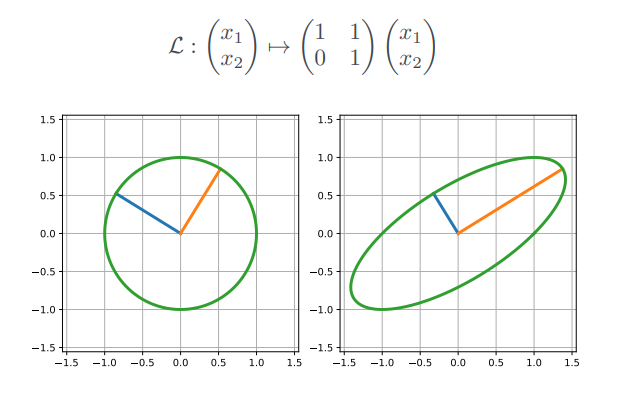
\includegraphics[scale=0.5]{assets/condition_number.png}
\end{center}
The green line is $\{x : ||x|| =1\}$

So the orange line would be the operator norm, given that it's the 'maximum stretch' of $||L||$.

The blue line is the 'minimum stretch' of $||L||$, or the 'maximums tretch of $||L^{-1}||$
\subsubsection{Storing the right-hand side $b$}

Perturbing $b \to b + \Delta b$ shifts the solution by $\Delta x = A^{-1}\Delta b$.
Bounding the numerator and denominator of the relative output error separately:
\[
  \|\Delta x\| = \|A^{-1}\Delta b\| \leq \|A^{-1}\|\cdot\|\Delta b\|,
  \qquad
  \|b\| = \|Ax\| \leq \|A\|\cdot\|x\|,
\]
the second inequality giving $\tfrac{1}{\|x\|} \leq \tfrac{\|A\|}{\|b\|}$.
Combining:
\[
  \frac{\|\Delta x\|}{\|x\|} \leq \|A^{-1}\|\cdot\|\Delta b\|\cdot\frac{\|A\|}{\|b\|}
  = \underbrace{\|A^{-1}\|\cdot\|A\|}_{k_{\mathrm{rel}}(A)}\cdot\frac{\|\Delta b\|}{\|b\|}.
\]
where we used $k_{\mathrm{rel}}(A^{-1}) = \|A^{-1}\|\cdot\|(A^{-1})^{-1}\|
= \|A^{-1}\|\cdot\|A\| = k_{\mathrm{rel}}(A)$.

\subsubsection{Perturbing the coefficient matrix $A$}

Consider storing irrational entries (e.g.\ $\sqrt{2}$) --- machine rounding
introduces a perturbation $\Delta A$.  The perturbed system is
\[
  (A + \Delta A)(x + \Delta x) = b + \Delta b.
\]

\paragraph{Claim.}
If $A$ is regular and $\|\Delta A\| < \tfrac{1}{\|A^{-1}\|}$,
then $A + \Delta A$ is also regular.

Geometrically: $\tfrac{1}{\|A^{-1}\|}$ is the smallest singular value of $A$
(the semi-minor axis of the image ellipsoid), while $\|\Delta A\|$ bounds the
size of the perturbation ellipsoid.  As long as the perturbation does not
exceed this minimum stretch, the perturbed map remains injective.

\paragraph{Proof.}
We show $(A + \Delta A)x \neq 0$ for all $x \neq 0$.
Suppose for contradiction that $(A + \Delta A)x = 0$.  Then
\[
  Ax = -\Delta A\,x
  \;\Longrightarrow\;
  x = -A^{-1}\Delta A\,x,
\]
so taking norms,
\[
  \|x\| = \|A^{-1}\Delta A\,x\|
        \leq \|A^{-1}\|\cdot\|\Delta A\|\cdot\|x\|
        < \|x\|,
\]
a contradiction (based on that $\| \Delta A\| < \frac{1}{\| A^{-1}\|}$).  Hence $A + \Delta A$ is injective, and since it is square,
it is regular. $\square$

\paragraph{Error bound.}
Under the conditions above the solution $\tilde{x} = x + \Delta x$ of
$(A + \Delta A)(x + \Delta x) = b + \Delta b$ satisfies
\[
  \underbrace{\frac{\|\Delta x\|}{\|x\|}}_{\text{relative output error}}
  \;\leq\;
  \underbrace{\frac{k_{\mathrm{rel}}(A)}{1 - k_{\mathrm{rel}}(A)\,\tfrac{\|\Delta A\|}{\|A\|}}}_{\text{amplification factor}}
  \cdot
  \underbrace{\left(\frac{\|\Delta A\|}{\|A\|}
              + \frac{\|\Delta b\|}{\|b\|}\right)}_{\text{relative input error}}.
\]
The denominator satisfies
$k_{\mathrm{rel}}(A)\tfrac{\|\Delta A\|}{\|A\|}
 = \|A^{-1}\|\cdot\|\Delta A\| < 1$
by assumption, so the bound is finite.
As $\|\Delta A\|$ approaches the regularity threshold $\tfrac{1}{\|A^{-1}\|}$
the denominator tends to zero and the amplification diverges --- a
near-singular $A + \Delta A$ can blow up any input error.
Given only the input data and its perturbations, this bound lets us
estimate the output error without knowing the true solution.

\subsection{Residual}
\subsubsection{Definition}

Numerical solution of $Ax = b$ yields an approximate $\tilde{x} = x + \Delta x$
with $A\tilde{x} \neq b$ in general.  The \textbf{residual} of $\tilde{x}$ is
\[
  \tilde{r} := b - A\tilde{x} = Ax - A(x + \Delta x) = -A\,\Delta x.
\]

\subsubsection{Error estimation}

From $\tilde{r} = -A\,\Delta x$ and $\Delta x = -A^{-1}\tilde{r}$,
\[
  \|\tilde{r}\| \leq \|A\|\cdot\|\Delta x\|,
  \qquad
  \|\Delta x\| \leq \|A^{-1}\|\cdot\|\tilde{r}\|,
\]
giving the two-sided bound
\[
  \frac{1}{\|A^{-1}\|}\|\Delta x\|
  \;\leq\; \|\tilde{r}\|
  \;\leq\; \|A\|\cdot\|\Delta x\|.
\]
When $A$ is well-conditioned, the two sides are close and a small residual
implies a small error.

Equivalently, $\tilde{x}$ is the \emph{exact} solution of a perturbed system:
\[
  A\tilde{x} = b - \tilde{r},
\]
so the only error is the unavoidable perturbation $\tilde{r}$ in the
right-hand side.  A solver is numerically stable precisely when it produces
solutions with small residuals.

\paragraph{Iterative refinement.}
If $\|\tilde{r}\|$ is acceptably small, we are done.  Otherwise:
\begin{enumerate}
  \item Compute the residual $\tilde{r} = b - A\tilde{x}$.
  \item Solve $A\,\delta x = \tilde{r}$ for the correction $\delta x$.
        (Since $A$ is already factored, e.g.\ via LU, this is cheap.)
  \item Update $\tilde{x} \leftarrow \tilde{x} + \delta x$ and return to step 1.
\end{enumerate}

\subsection{QR Decomposition}
Instead of decomposing $A = LR$, we decompose $A = QR$, where $Q$ is orthogonal and $R$ is an upper triangular matrix.

\subsubsection{Orthogonal Vectors and Matrices}
We work in $\mathbb{R}^n$ with the scalar product $\langle u,v \rangle := u^T v$ and the Euclidean norm $\|v\|_2 = \sqrt{v^T v}$.

Two vectors $u$, $v$ are \textbf{orthogonal} if $\langle u,v \rangle = 0$.

A system $\{v_1,\dots,v_k\}$ of vectors is \textbf{orthogonal} if all pairs are mutually orthogonal, and \textbf{orthonormal} if additionally $\|v_i\|_2 = 1$ for all $i$.

A matrix $Q\in \mathbb{R}^{n\times n}$ is \textbf{orthogonal} if $Q^TQ = QQ^T = I$.

\paragraph{Orthogonal transformations preserve Euclidean length:}
\[
\|Qx\|_2^2 = (Qx)^T(Qx) = x^TQ^TQx = x^TIx = x^Tx = \|x\|_2^2
\]

\paragraph{Determinant of orthogonal matrices:} Orthogonal matrices always have determinant $\pm 1$:
\[
1 = \det(I) = \det(Q^TQ) = \det(Q^T)\cdot\det(Q) = \det(Q)^2
\implies \det(Q) = \pm 1
\]

\paragraph{Examples of orthogonal matrices:}
\begin{itemize}
  \item The identity matrix $I$.

  \item \textbf{Transposition matrix} $P_{j,j'}$: the identity matrix with an additional $1$ at positions $(j,j')$ and $(j',j)$ (i.e., two rows/columns are swapped).

  \item \textbf{Permutation matrix}: a product of transposition matrices. This follows from the fact that the product of two orthogonal matrices is orthogonal: given $Q_1^TQ_1 = I$ and $Q_2^TQ_2 = I$,
  \[
  (Q_1Q_2)^T(Q_1Q_2) = Q_2^TQ_1^TQ_1Q_2 = Q_2^TQ_2 = I.
  \]
\end{itemize}

\subsubsection{Rotation Matrices in $\mathbb{R}^{2\times 2}$}
Let $s, c \in [-1,1]$ with $s^2 + c^2 = 1$ describe an angle $\phi \in [0,2\pi)$ via $s = \sin(\phi)$ and $c = \cos(\phi)$. The following matrix describes a rotation by $\phi$:
\[
G =
\begin{bmatrix}
  c  & s \\
  -s & c
\end{bmatrix}
\]
We verify that $G$ is orthogonal by checking its columns $[c,\,-s]^T$ and $[s,\,c]^T$:
\begin{itemize}
  \item \textbf{Orthogonality:} $[c,\,-s]\cdot[s,\,c]^T = cs - sc = 0$ \checkmark
  \item \textbf{Unit norm:} $\|[c,\,-s]^T\|_2 = \|[s,\,c]^T\|_2 = \sqrt{c^2+s^2} = 1$ \checkmark
\end{itemize}

\subsubsection{Generalization: Givens Rotation Matrix}
\label{sec:givens}
The rotation above applies to 2D vectors. The Givens matrix $G_{j,i}(c,s) \in \mathbb{R}^{n\times n}$ generalizes this to arbitrary dimensions by embedding the $2\times 2$ rotation into an otherwise identity matrix, acting on rows $i$ and $j$.

\begin{center}
  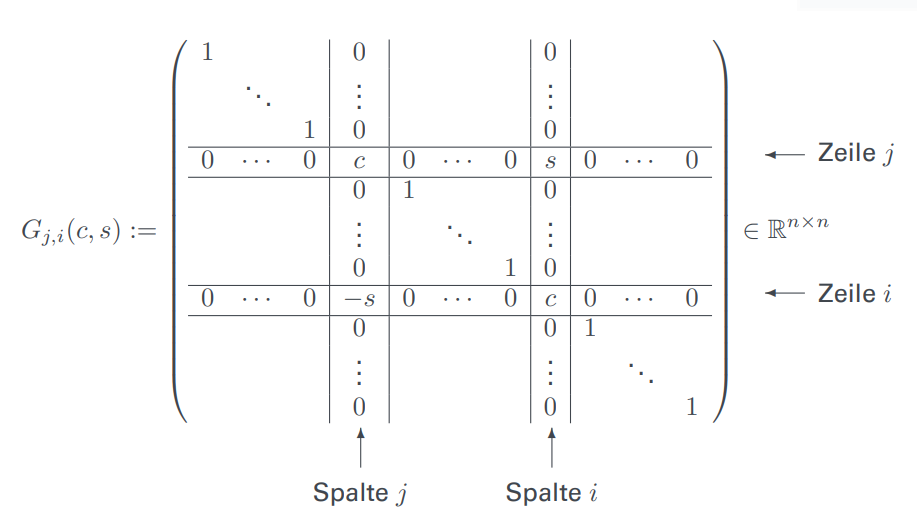
\includegraphics[scale=0.5]{assets/rotation_matrix.png}
\end{center}

Note: the function is written $G_{j,i}$, not $G_{i,j}$ — this convention should be taken as given.

\paragraph{Comparison of $G_{j,i}(c,s)$ and $L_{i,j}(\alpha)$:}
Left-multiplying by $L_{i,j}(\alpha)$ subtracts $\alpha$ times row $j$ from row $i$. In contrast, left-multiplying by $G_{j,i}(c,s)$ mixes rows $i$ and $j$ as follows:
\[
\text{row}_i \leftarrow c\cdot\text{row}_i - s\cdot\text{row}_j, \qquad
\text{row}_j \leftarrow s\cdot\text{row}_i + c\cdot\text{row}_j
\]

In Python:
\begin{lstlisting}[language=Python]
def G_multiplied_A(j, i, c, s, A):
    for k in range(n):
        temp   = A[i][k]
        A[i][k] = c * temp    - s * A[j][k]
        A[j][k] = s * temp    + c * A[j][k]
        # Note: temp saves the old A[i][k] before it is overwritten
\end{lstlisting}

Our goal is to choose $c$ and $s$ such that $a_{i,j}$ becomes zero after the transformation:
\[
a_{i,j} = 0, \qquad
s = \frac{a_{i,j}^{\text{old}}}{\rho}, \qquad
c = \frac{a_{j,j}^{\text{old}}}{\rho}, \qquad
\rho = \pm\sqrt{\left(a_{j,j}^{\text{old}}\right)^2 + \left(a_{i,j}^{\text{old}}\right)^2}
\]
This choice ensures $s^2 + c^2 = 1$.

\subsubsection{QR Decomposition via \hyperref[sec:givens]{Givens} Rotations}
The idea is that all Givens matrices are orthogonal, and we make it so that through $G_{j,i}$ we make A a triangular matrix $R$. So we have
\[QA = R \Rightarrow A = Q^TR\]



\begin{lstlisting}
for j = 1, ..., n-1:
    for i = j+1, ..., n:
        // Eliminate a_{i,j}, analogously to LR decomposition
        rho_{i,j} := pm sqrt(a_{j,j}^2 + a_{i,j}^2)
        c_{i,j}   := a_{j,j} / rho_{i,j}
        s_{i,j}   := a_{i,j} / rho_{i,j}
        A         <- G_{j,i}(c_{i,j}, s_{i,j}) * A
\end{lstlisting}

After all iterations, we have $Q^T = G_{n-1,n}\cdots G_{j,i} \cdots G_{1,2}$, so that:
\[
R = Q^T A \implies A = QR
\]
(Moving $Q^T$ to the other side uses orthogonality: $Q^{-1} = Q^T$, so $QQ^T = I$.)


Each matrix $A\in\mathbb{R}^{m\times n}$

To solve $Ax = b$, we then solve the two simpler steps:
\[
y = Q^T b, \qquad Rx = y
\]

\subsection{QR vs LR Decomposition}
QR decomposition is generally about twice as expensive as LR.

The elimination of $a_{i,j}$ requires $\rho_{i,j} \neq 0$. If $\rho_{i,j} = 0$, then $a_{i,j} = 0$ already and there is nothing to do — this is handled by a simple \texttt{if} check.

Unlike LR, \textbf{QR decomposition does not require $A$ to be invertible (regular)}.

QR decomposition also extends naturally to rectangular matrices $A \in \mathbb{R}^{m\times n}$ with $m > n$. Simply adjust the loop bounds:
\begin{lstlisting}
for j = 1, ..., n:    // upper limit changes from n-1 to n
    for i = j+1, ..., m:  // m instead of n
\end{lstlisting}

\subsection{Singular Value Decomposition (SVD)}
SVD is less commonly used for solving linear systems $Ax = b$. Instead, the focus shifts to computing the action of $A$: given $x$, compute $Ax$.

Every matrix $A \in \mathbb{R}^{m\times n}$ admits a decomposition:
\[A = U\Sigma V^T\]
where:
\begin{itemize}
  \item $U \in \mathbb{R}^{m\times m}$ is orthogonal,
  \item $\Sigma = \operatorname{diag}(\sigma_1, \dots, \sigma_p) \in \mathbb{R}^{m\times n}$, with $p = \min(m,n)$ and $\sigma_1 \geq \sigma_2 \geq \cdots \geq \sigma_p \geq 0$,
  \item $V \in \mathbb{R}^{n\times n}$ is orthogonal.
\end{itemize}

Assuming $n \leq m$, let $u_1, \dots, u_n$ be the first $n$ columns of $U$ and $v_1, \dots, v_n$ be the columns of $V$. Then:
\[
A = U\Sigma V^T = \sum_{i=1}^{n} \sigma_i \underbrace{u_i v_i^T}_{\in\,\mathbb{R}^{m\times n}}
\]

The map $x \mapsto Ax$ can be understood in three steps:
\begin{enumerate}
  \item $x \mapsto V^T x$: project $x$ onto the basis given by the columns of $V$ (orthogonal change of basis),
  \item $V^T x \mapsto \Sigma V^T x$: scale the $i$-th component by $\sigma_i$,
  \item $\Sigma V^T x \mapsto U\Sigma V^T x$: rotate/reflect into the output space via $U$.
\end{enumerate}
Since $U$ and $V$ are orthogonal (norm-preserving), the singular values $\sigma_i$ entirely determine how much each direction is stretched or compressed.

\subsubsection{Rank-$r$ Approximation}
Since $\sigma_1 \geq \sigma_2 \geq \cdots \geq \sigma_n \geq 0$, if $\sigma_{r+1}$ is sufficiently small for some $r \in \mathbb{N}$, we can truncate the sum:
\[
A = \sum_{i=1}^{n} \sigma_i u_i v_i^T \approx \tilde{A} := \sum_{i=1}^{r} \sigma_i u_i v_i^T
\]
If $r \ll n$, this yields a major reduction in both storage and computation.

\paragraph{Example: document-word matrices.}
Given $m$ documents and $n$ unique words, define $A_{i,j}$ as the frequency of word $j$ in document $i$. Since this matrix is queried very frequently, we compute the SVD of $A$ once (the expensive step) and then work with the rank-$r$ approximation $\tilde{A}$. This is efficient as long as only a few singular values are significant.

\section{Linear Curve Fitting (Lineare Ausgleichsrechnung)}
% "Lineare Ausgleichsrechnung" translates directly to "Linear Least Squares" or
% "Linear Curve Fitting". Both are standard English terms for this topic.
% For clickable links throughout the document, add to your preamble:
% \usepackage[colorlinks=true, linkcolor=blue, urlcolor=blue]{hyperref}

\subsection{Refresher}
With systems of linear equations we had $Ax = b$, where $A \in \mathbb{R}^{n\times n}$
and $x, b \in \mathbb{R}^n$, along with the concept of the \textbf{residual}.

For an approximate solution $\tilde{x} \in \mathbb{R}^n$, we measure how good it is via:
$\tilde{r} := b - A\tilde{x}$
\begin{itemize}
  \item $\tilde{r} = 0$: $\tilde{x}$ is the exact solution
  \item $\|\tilde{r}\|$ small: acceptable approximation
\end{itemize}

\subsection{Refresher: Regression}
For data points $(x_i, y_i)$ we model:
\[y_i \approx \alpha + \beta \cdot x_i\]
This can be written as a linear system:
\[
\begin{bmatrix} 1 & x_1 \\ \vdots & \vdots \\ 1 & x_m \end{bmatrix}
\begin{bmatrix} \alpha \\ \beta \end{bmatrix}
=
\begin{bmatrix} y_1 \\ \vdots \\ y_m \end{bmatrix}
\]
We want to minimize the sum of squared residuals:
\[Q(\alpha,\beta) = \sum_{i=1}^{m}\epsilon_i^2 = \|\tilde{r}\|_2^2\]

\subsection{Linear Curve Fitting}
We have:
\begin{itemize}
  \item $A \in \mathbb{R}^{m \times n}$ with $m \geq n$ (more equations than unknowns)
        and $\mathrm{rank}(A) = n$ (columns are linearly independent)
  \item $x \in \mathbb{R}^n$, $b \in \mathbb{R}^m$
\end{itemize}
The mapping $x \mapsto Ax$ spans an $n$-dimensional subspace of $\mathbb{R}^m$, so
$Ax = b$ may have no exact solution.

We therefore look for the \textbf{best approximation} $x^* \in \mathbb{R}^n$ such that:
\[
  \|Ax^* - b\|_2 = \min_{x \in \mathbb{R}^n} \|Ax - b\|_2
\]
i.e.\ we minimize the Euclidean norm of the residual $\tilde{r} = b - Ax$.

\subsection{Solving with the Normal Equation}
We want to minimize:
\[f : \mathbb{R}^n \to \mathbb{R}, \qquad f(x) := \|Ax - b\|_2^2\]
Strategy: set the gradient $\nabla f$ to zero, then verify the Hessian is
positive definite (guaranteeing a minimum).

\paragraph{Expanding $f$:}
\[
  f(x) = \|Ax-b\|_2^2 = (Ax-b)^T(Ax-b) = (x^TA^T - b^T)(Ax - b)
\]
\[
  = x^TA^TAx - x^TA^Tb - b^TAx + b^Tb
\]
\textbf{Note:} Every term is a scalar $\in \mathbb{R}$, so we can freely transpose any of them.
The second and third terms are transposes of each other and therefore equal:
\[
  = x^TA^TAx - 2x^TA^Tb + b^Tb
\]

\paragraph{Directional derivative:}
For a direction vector $h \in \mathbb{R}^n$:
\[
  D_h f(x) = \lim_{\epsilon \to 0} \frac{f(x + \epsilon h) - f(x)}{\epsilon}
\]

\paragraph{Computation on the side:}
\[
  f(x + \epsilon h) - f(x)
\]
\[
  \text{(first part):}\quad (x+\epsilon h)^T A^TA(x+\epsilon h) - x^TA^TAx
\]
\[
  \text{(second part):}\quad -2(x+\epsilon h)^TA^Tb + 2x^TA^Tb
\]
\[
  \text{(third part):}\quad b^Tb - b^Tb = 0
\]
Combined:
\[
  = \epsilon h^TA^TAx + \epsilon x^TA^TAh + \epsilon^2 h^TA^TAh - 2\epsilon h^TA^Tb
\]
Dividing by $\epsilon$ and taking the limit (the $\epsilon^2$ term vanishes):
\[
  D_h f(x) = \underbrace{2h^TA^TAx}_{\text{two equal terms joined by transposition}}
             - 2h^TA^Tb = h^T\!\left(2A^TAx - 2A^Tb\right)
\]

\paragraph{Gradient:}
The gradient $\nabla f(x)$ is the unique vector satisfying $D_h f(x) = h^T \nabla f(x)$
for \emph{all} $h \in \mathbb{R}^n$. Reading off from the expression above:
\[
  \nabla f(x) = 2(A^TAx - A^Tb)
\]
Recall that the gradient collects all partial derivatives:
\[
  \nabla f = \begin{bmatrix} \tfrac{\partial f}{\partial x_1} \\ \vdots \\
             \tfrac{\partial f}{\partial x_n} \end{bmatrix}
\]
Setting $\nabla f = 0$ gives the \textbf{Normal Equation}:
\[
  \nabla f = 0 \;\Longleftrightarrow\; A^TAx^* = A^Tb
\]

\paragraph{Verifying it is a minimum:}
The Hessian is $H_f = 2A^TA$. It is positive definite because:
\[
  \forall\, x \neq 0 \in \mathbb{R}^n : \quad
  x^T(A^TA)x = (Ax)^T(Ax) = \|Ax\|_2^2 > 0
\]
\begin{itemize}
  \item $\geq 0$: always true since it is a squared norm
  \item $> 0$: because $\mathrm{rank}(A) = n$ means $A$ has a trivial null space,
        so $Ax = 0 \Rightarrow x = 0$. Therefore $x \neq 0 \Rightarrow Ax \neq 0
        \Rightarrow \|Ax\|_2^2 > 0$
\end{itemize}

\textbf{Conclusion:} The Normal Equation $A^TAx^* = A^Tb$ has a unique solution $x^*$
which is the global minimum.

\paragraph{Computing costs:}
\begin{itemize}
  \item $A^TA$: $\mathcal{O}(mn^2)$
  \item $A^Tb$: $\mathcal{O}(mn)$
  \item Solving the system: $\mathcal{O}(n^3)$
\end{itemize}

\paragraph{Geometrical interpretation:}
For any $y \in \mathbb{R}^n$, the optimal residual $\tilde{r}^* = b - Ax^*$ is
orthogonal to the column space of $A$:
\[
  \langle Ay, \tilde{r}^* \rangle
  = (Ay)^T \tilde{r}^*
  = y^T A^T \tilde{r}^*
  = y^T A^T (b - Ax^*)
  = y^T \underbrace{(A^Tb - A^TAx^*)}_{=\,0}
  = 0
\]
The residual is \textbf{perpendicular} to every vector in the image of $A$.

\paragraph{Example:}
\[
  A = \begin{bmatrix} 2 \\ 1 \end{bmatrix}, \quad
  b = \begin{bmatrix} 2 \\ 6 \end{bmatrix}
\]
\[
  A^TA = [5], \quad A^Tb = [10], \quad x^* = [2], \quad
  Ax^* = \begin{bmatrix} 4 \\ 2 \end{bmatrix}, \quad
  \tilde{r}^* = \begin{bmatrix} -2 \\ 4 \end{bmatrix}
\]
\begin{center}
  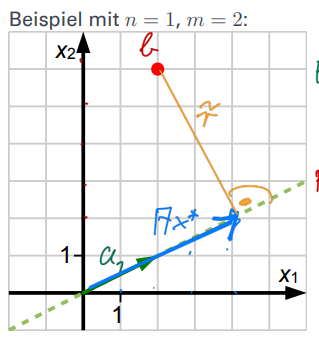
\includegraphics[scale=0.5]{assets/geometrical_interpretation_normalequation.png}
\end{center}

\subsection{Alternative Method: Triangular Matrix}
If $A$ is already an upper triangular matrix $R$, all diagonal entries must be nonzero
(otherwise $\mathrm{rank}(A) < n$).

Minimizing $\|Rx - b\|_2^2$ is then easy:
\begin{itemize}
  \item The first $n$ rows can be solved exactly $\Rightarrow$ residual is zero there
  \item The remaining rows below row $n$ are all zero in $R$, so they contribute
        $-b_i$ to the residual and cannot be reduced further
\end{itemize}

\subsection{Solving with QR-Decomposition}
For an orthogonal matrix $Q$, multiplying by $Q^T$ preserves the Euclidean norm
($Q^TQ = I$):
\[
  \|Ax - b\|_2 = \|Q^TAx - Q^Tb\|_2
\]
Since the QR-decomposition gives $Q^TA = R$, we reduce to the triangular case above
and solve $\|Rx - Q^Tb\|_2$.

\paragraph{Costs:}
\begin{itemize}
  \item QR-decomposition: $\mathcal{O}(mn^2)$
  \item Solving: $\mathcal{O}(n^3)$
\end{itemize}
Same asymptotic cost as the normal equation, but \textbf{numerically more stable}.

\paragraph{Example} (same data as before):
\[
  A = \begin{bmatrix} 2 \\ 1 \end{bmatrix}
\]
We apply a \hyperref[sec:givens]{Givens rotation} to zero out the second entry of $A$.
The rotation parameters are:
\begin{itemize}
  \item $\rho = \|A\|_2 = \sqrt{2^2 + 1^2} = \sqrt{5}$ \quad (norm of the column,
        becomes the diagonal entry of $R$)
  \item $c = \tfrac{2}{\sqrt{5}}$ \quad (cosine of the rotation angle)
  \item $s = \tfrac{1}{\sqrt{5}}$ \quad (sine of the rotation angle)
\end{itemize}
\[
  G = \frac{1}{\sqrt{5}}\begin{bmatrix} 2 & 1 \\ -1 & 2 \end{bmatrix}
\]
\[
  \underbrace{G}_{=Q^T} \cdot A
  = \frac{1}{\sqrt{5}}\begin{bmatrix} 5 \\ 0 \end{bmatrix} = R
  \qquad
  Q^Tb = \frac{1}{\sqrt{5}}\begin{bmatrix} 10 \\ 10 \end{bmatrix}
\]
Solving the first (only nonzero) row of $Rx^* = Q^Tb$:
\[
  \frac{5}{\sqrt{5}}\, x^* = \frac{10}{\sqrt{5}}
  \;\Longrightarrow\; 5x^* = 10
  \;\Longrightarrow\; x^* = 2
\]
This matches the result from the normal equation.

\paragraph{Geometrical interpretation:}
With $A = QR$ and $Q$ orthogonal:
\begin{itemize}
  \item $x^*$ is determined by the first $n$ rows of $Rx^* = Q^Tb$
  \item The residual $Q^Tb - Rx^*$ has zeros in the first $n$ entries
        and free values in the rest:
\end{itemize}
\[
  Q^Tb - Rx^* = \begin{bmatrix} 0 \\ \vdots \\ 0 \\ \ast \\ \vdots \end{bmatrix}
  \qquad
  Ry = \begin{bmatrix} \ast \\ \vdots \\ \ast \\ 0 \\ \vdots \end{bmatrix}
\]
These two vectors are trivially orthogonal (nonzero parts never overlap). Undoing
the $Q^T$ transformation:
\[
  Q^Tb - Rx^* \perp Ry
  \;\Longleftrightarrow\; b - QRx^* \perp QRy
  \;\Longleftrightarrow\; b - Ax^* \perp Ay
\]
So the residual is orthogonal to the image of $A$ — same conclusion as before.

\subsection{Uses of This}

\subsubsection{Linear Models}
We can fit not just lines but any model that is \emph{linear in the unknowns}.
For example, fitting a quadratic:
\[y_i \approx \alpha + \beta x_i + \gamma x_i^2\]
\[
\begin{bmatrix}
  1 & x_1 & x_1^2 \\
  \vdots & \vdots & \vdots \\
  1 & x_m & x_m^2
\end{bmatrix}
\begin{bmatrix} \alpha \\ \beta \\ \gamma \end{bmatrix}
=
\begin{bmatrix} y_1 \\ \vdots \\ y_m \end{bmatrix}
\]
The unknowns $\alpha, \beta, \gamma$ appear linearly, so the same least-squares
machinery applies directly.

\section{Function Representation}
\subsection{Interpolation}

\subsubsection{Basic introduction}
Given we have a function $f(x)$, and we know the value of the function at two points $f(x_0)$, $f(x_1)$. We then try to 'guess' the value of a third value in the middle $f(x)$. We can attempt to draw a straight line to connect the points, or some better techniques.

But however we also refer to the term interpolation as bringing a function into our computer.

So in our computer a number $x\in\mathbb{R}$ is mapped onto a $\tilde{x}\in\mathbb{F}_{B,t,\alpha\beta}$ (remember floating point systems)

So our function $f$ in the computer is represented as a $\tilde{f} \approx f$

An example of this would be: input is a photo and the output is 'is it a cat?'.

But in general for our usecase we are limiting ourselves for f to be $f:\mathbb{R}\to\mathbb{R}$ (no multiple dimensions). We are also limiting ourselves to linear combinations of response functions, determined by
linear functionals

\subsubsection{Concept of 'interpolation'}
There are two possible definitions:
\begin{enumerate}
  \item Compute the approximation $\tilde{f}$
  \item Given points $(x_0,f(x_0)),\dots,(x_n,f(x_n))$ (called \textbf{bases}) and a 
  \[x \in \left[\min_{0\leq i \leq n}(x_i) , \max_{0\leq i \leq n}(x_i)\right]\]
  compute the $\hat{f}(x)$

  When the $x$ is not in that range, we call that extrapolation.
\end{enumerate}

\subsection{Linear Functionals}
\subsubsection{Functions as Vectors}
For a body $\mathbb{K}$ and a definition domain X with $\emptyset \neq X \subseteq \mathbb{K}$ we define
\[G := \{f:X \to \mathbb{K}\}\]
as a $\mathbb{K}$\textbf{-Vector space} closed under
\begin{itemize}
  \item Addition $f+g: x \to f(x) + g(x) \quad f,g\in G, x\in X$
  \item Scalar multiplication: $\alpha f: x\to \alpha f(x) \quad f\in G, \alpha\in\mathbb{K}, x\in X$
\end{itemize}

The Vector axioms are followed (we believe without proof)

\paragraph{Approximation}: We pick a finite-dimensional subspace $G_n$ with $\dim G_n = n+1$. This $G_n$ can be defined as all polynomials of degree at most $n$, but represented with a basis instead of $x^j$

As an example, $X := \mathbb{K} := \mathbb{R}$ and $G_2$ is $x\to \alpha x^2 + \beta x + \gamma$ with $\alpha,\beta,\gamma \in \mathbb{R}$

Usually we pick a Basis $\phi_0,...,\phi_n \in G_n$

Example: For $G_2$ we can pick $\phi_0 : x\to 1$, $\phi_1: x \to x$, $\phi_2: x\to x^2$ as our base.

And then we formulate linear conditions to determine $\tilde{f} \in G_n$. This is usually formulated as coefficients for the basis.

\subsubsection{Linear Functionals}
For a $\mathbb{K}$-Vector space V, the linear Mapping $V\to \mathbb{K}$ is called \textbf{Linear Functional}

So for $V = \mathbb{R}^2$ we can define for example
\[\mu_1 :\begin{pmatrix}
  x_1\\
  x_2
\end{pmatrix} \to x_2  = \begin{bmatrix}
  0 & 1
\end{bmatrix}\begin{bmatrix}
  x_1\\
  x_2
\end{bmatrix}\quad \mu_2: \begin{pmatrix}
  x_1 \\
  x_2
\end{pmatrix}\to x_1 + x_2 = \begin{bmatrix}
  1 & 1
\end{bmatrix}\begin{bmatrix}
  x_1\\
  x_2
\end{bmatrix}\]

We usually assume that the Functional $\mu$ is not the null function. Then

\paragraph{Linear Functionals for the Function space $G_n$}: 

These are all linear functionals that take a function and return a number, we just believe it.
\begin{enumerate}
  \item Analysis in $x^*$: $\mu_{aus,x^*}:g\to g(x^*)$
  \item Analysis of the derivate in $x^*$: $\mu_{abl,x^*}: g\to g'(x^*)$
  \item Integral over the definition Domain X
  \[\mu_{int}(g) := \int_X g(t)dt\]
  \item \dots (there are many more, such as linear combinations of these)
\end{enumerate}

\subsubsection{Matrix Representation through Basis}
Function Space $G_n$ with dimension $n+1$ and the Basis $(\phi_0,\dots,\phi_n)$

\[G_n \ni g = \sum_{j=0}^{n}\alpha_j \cdot \phi_j\]
For functionals $\mu_0,...,\mu_n$
\[y_i = \mu_i(g) = \mu_i\left(\sum_{j=0}^{n}\alpha_j \cdot \phi_j\right) \underbrace{=}_{\text{linear}} \sum_{j=0}^{n}\underbrace{\alpha_j}_{\text{Unknown}}\underbrace{\mu_i(\phi_j)}_{\text{Known}}\]

So this maps out to a System of Linear Equations
\begin{center}
  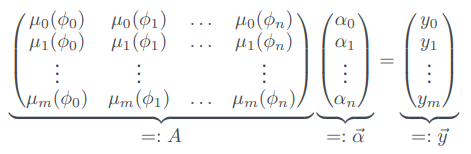
\includegraphics[scale=0.7]{assets/linear_functionals_matrix.png}
\end{center}
This $A$ is called the \textbf{Interpolation matrix}, dependant on linear functions $\mu_i$ and basis $\phi_j$

\paragraph{'Hau-Ruck Method'}: (named by the professor)

Here $n = m$. We pick our functionals $\mu_i$, our right hand sides $y_i$ and our bases $\phi_i$. We set up the interpolation matrix A (which is done in $O(n^2)$)

Solve the System of Linear Equations $\to \alpha_0,...,\alpha_n \to g = \sum \alpha_j\phi_j$ in $O(n^3)$

\paragraph{Example}: Given $g\in \Pi_2$ so polynoms with degree $\leq 2$

\begin{center}
  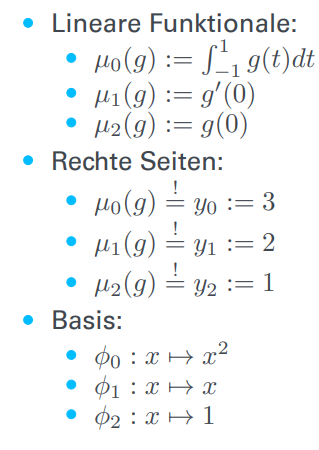
\includegraphics[scale=0.5]{assets/interpolation_problem_example.png}
\end{center}
The solution for this can be computed by myself.

\subsection{Polynomials}
We define polynoms of degree at most $n \in \mathbb{N}_0$
\[\Pi_n := \left\{f:\mathbb{K}\to\mathbb{K} : \exists a_0,...,a_n\in\mathbb{K}: \forall x \in \mathbb{K} :f(x) = \sum_{j=0}^na_jx^j\right\}\]

So all Polynomials
\[\Pi := \bigcup_{n=0}^{\infty}\Pi_n\]

Degree of $p \in \Pi \backslash \{0\}$
\[Deg(p) := \min\{n\in \mathbb{N}_0 : p\in \Pi_n\}\]
Note: $Deg(0) := -\infty$

And then $\Pi_n$ and $\Pi$ are vector spaces with 
\[\Pi_n  = \text{span}\{x\to 1, x\to x, x\to x^2,\dots,x\to x^n\}\]

\subsubsection{Dividing by zero / Splitting off roots}
For $p \in \Pi \backslash \{0\}$ with $p(x_0) = 0$
\[p(x) = (x-x_0)q(x) \quad Deg(q) < Deg(p)\]

\paragraph{Example}: $p(x) = x^3-x \quad x_0 = 1$

So $x^3 - x = (x-1)(x^2+x)$

From this we follow that
\begin{itemize}
  \item Polynomials $p\in\Pi \backslash \{0\}$ can have at most $Deg(p)$ null points
  \item If two polynomials $p$ and $q$ from $\Pi_n$ match at $n+1$ points then they are equal.
\end{itemize}

\subsubsection{Principle of the Coefficient comparison}
If a polynomial $p \in \Pi_n$ is known on a set $X \subset \mathbb{K}$ that contains at least $n + 1$ points, it can be uniquely represented as:
\[p(x) = \sum_{j=0}^n a_j x^j\]

Specifically:
\begin{itemize}
  \item For $n < |\mathbb{K}|$ and $p \in \Pi_n$, the coefficients $a_j$ ($0 \leq j \leq n$) are uniquely determined.
  \item Even more specifically: Then $a_n$ is uniquely determined. For $Deg(p) = n$, it holds that $a_n \neq 0$ (otherwise $Deg(p) < n$). This $a_n$ is called the \textbf{Leitkoeffizient} of $p$.
  \item From this, the monoms $x \mapsto 1, x \mapsto x, x \mapsto x^2, \dots, x \mapsto x^n$ form a valid basis of $\Pi_n$.
\end{itemize}
From now on, we always assume $n < |\mathbb{K}|$ (usually thinking of $\mathbb{K} = \mathbb{R}$).
\subsection{Lagrange Interpolation}
We are going to specialize ourselves with the following parameters:
\begin{itemize}
  \item $m=n$
  \item $G_n := \Pi_n$. We are using polynomials of degree at most $n$.
  \item Linear functionals defined by evaluation at a point:
  \[\mu_i := \mu_{aus,x_i} : g \to g(x_i)\]
  for $n+1$ distinct support points $x_0,...,x_n \in \mathbb{K}$.
  \item Target values $y_i = f(x_i)$ for $0\leq i \leq n$, where $f$ is the function to interpolate.
\end{itemize}

\paragraph{Note}: Through $n+1$ distinct support points, we can determine a unique interpolation polynomial $p\in \Pi_n$.

The uniquely determined polynomial $g\in\Pi_n$ satisfying $\mu_i(g) = \mu_i(f) \, \forall i$ is called the \textbf{Lagrange interpolation polynomial}, denoted as:
\[P(f|x_0,...,x_n)\]
Thus, $g$ is the explicit interpolation function we aim to compute.

\subsubsection{Lagrange Interpolation Task: System of Linear Equations with Vandermonde Matrix}
If we select the standard monomial basis $\phi_j : x \to x^j$ from $\Pi_n$, the resulting interpolation matrix (recalling that $\mu_i := \mu_{aus,x_i}$) is configured as:
\begin{center}
  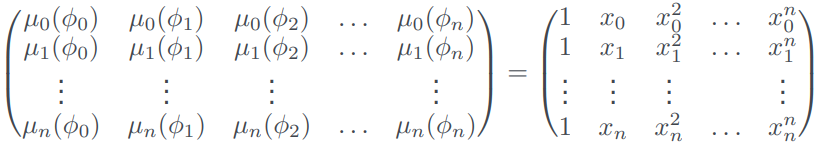
\includegraphics[scale=0.5]{assets/vandermonde_matrix.png}
\end{center}
This system matrix is called the \textbf{Vandermonde matrix}.

With it, we can determine the coefficients $\alpha_j$ to resolve:
\[P(f|x_0,...,x_n) = \sum_{j=0}^n\alpha_jx^j\]

While this matrix is regular (invertible), it is notoriously badly conditioned. Consequently, we require more numerically stable methods to determine $P(f|x_0,...,x_n)$.

\subsubsection{Lagrange Polynomials}

\paragraph{Prettiest interpolation matrix for the Lagrange interpolation task?}
The entries of our interpolation matrix are given by $\mu_i(\phi_j)$. Can we choose a basis such that the interpolation matrix simplifies directly to the Identity Matrix?

If so, the coefficients would map directly to $\alpha_j = f(x_j)$, yielding:
\[P(f|x_0,...,x_n) = \sum_{j=0}^n\underbrace{f(x_j)}_{\alpha_j}\phi_j\]
For this to hold, the basis functions $\phi_j$ must satisfy the Kronecker delta property under evaluation:
\[\mu_i(\phi_j) = \phi_j(x_i) = \begin{cases}
  1 \quad \text{if } i = j\\
  0 \quad \text{else}
\end{cases}\]
This formulation represents a valid Lagrange interpolation task with a unique solution. This specific basis polynomial is called the \textbf{Lagrange polynomial}, denoted as $l_{j,n}$.

\paragraph{Construction of the Lagrange Polynomial}: 
Since $l_{j,n}(x_i) = 0$ for all $i \neq j$, it possesses at least $n$ roots. This allows us to structure it as a product:
\[l_{j,n}(x) = q_j \prod_{i=0,i\neq j}^n(x-x_i)\]
Given the normalization condition $l_{j,n}(x_j) = 1$, the scaling constant must be:
\[q_j = \frac{1}{\prod_{i=0,i\neq j}^n (x_j - x_i)}\]
Combining these yields the complete formula for the Lagrange polynomials:
\[l_{j,n}(x) := \prod_{i=0,i\neq j}^n\frac{x-x_i}{x_j-x_i}\]

\begin{quote}
\textbf{Note:} A single $l_{j,n}(x)$ is not the final interpolating function; it is merely a constituent basis polynomial that equals 1 at its corresponding node and 0 at all others. The actual global interpolation polynomial is built via their linear combination:
\[L(x) = \sum_{j=0}^{n}y_jl_{j,n}(x)\]
\end{quote}

\subsubsection{Aitken-Neville-Strategy}
The Aitken-Neville scheme computes the full interpolation polynomial $P(f|x_0,...,x_n)$ progressively through a sequence of lower-degree \textbf{Help polynomials}:
\[P_{i,k} := P(f|x_{i-k},...,x_i)\]
Here, $P_{i,k}$ has a maximum degree of $k$ and interpolates at the support point $x_i$ along with its $k$ preceding points $x_{i-1},...,x_{i-k}$.

Our ultimate target value is $P_{n,n} = P(f|x_0,...,x_n)$. 
We can establish base cases at $k=0$ as constant functions: $P_{i,0}(x) = f(x_i)$.

The core idea is to recursively compute higher-order polynomials $P_{i,k}$ using the lower-order results $P_{i,k-1}$ and $P_{i-1,k-1}$:
\[P_{i,k}(x) = \frac{x-x_{i-k}}{x_i-x_{i-k}}P_{i,k-1}(x) + \frac{x_i-x}{x_i-x_{i-k}}P_{i-1,k-1}(x)\]

\paragraph{Verification of the Interpolation Properties:}
\begin{enumerate}
  \item \textbf{At point $x_i$}: $P_{i,k}(x_i) = 1 \cdot P_{i,k-1}(x_i) + 0 = f(x_i)$.
  \item \textbf{At point $x_{i-k}$}: $P_{i,k}(x_{i-k}) = 0 + 1 \cdot P_{i-1,k-1}(x_{i-k}) = f(x_{i-k})$.
  \item \textbf{At intermediate points $x_j$ ($i-k < j < i$)}: Both sub-polynomials successfully interpolate $f(x_j)$, resulting in:
  \[P_{i,k}(x_j) = \frac{x_j-x_{i-k} + x_i-x_j}{x_i-x_{i-k}} f(x_j) = f(x_j)\]
  Thus, it correctly interpolates across \textbf{all} target points in its window.
\end{enumerate}

This relationship yields the following triangular scheme algorithm:
\begin{algorithm}[H]
\begin{algorithmic}[1]
\For{$i = 0,\dots,n$}
  \State $P_{i,0} \leftarrow f(x_i)$
\EndFor
\For{$k = 1,\dots,n$}
  \For{$i = k,\dots,n$}
    \State $P_{i,k}(x) \leftarrow \frac{x-x_{i-k}}{x_i-x_{i-k}}P_{i,k-1}(x) + \frac{x_i-x}{x_i-x_{i-k}}P_{i-1,k-1}(x)$
  \EndFor
\EndFor
\State \textbf{Result:} $P_{n,n}$
\end{algorithmic}
\end{algorithm}

\paragraph{Optimizations:}
\begin{center}
  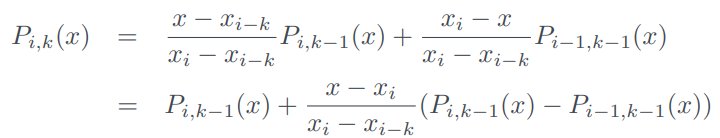
\includegraphics[scale=0.5]{assets/improvement_neville.png}
\end{center}
We can structurally eliminate redundant multiplications and minimize memory overhead by overwriting a single vector array row-by-row.

\textbf{Note:} If we only need to evaluate the interpolation function at one specific static point $x^*$, we run the algorithm directly on that scalar value instead of tracking full symbolic polynomials. This reduces operations purely to cheap scalar steps with a runtime complexity of $O(n^2)$.

\subsubsection{Newtonian Interpolation Formula}
While Neville's algorithm evaluates a single point efficiently in $O(n^2)$, the Newton formulation allows us to reconstruct the entire analytical polynomial expression explicitly within the same $O(n^2)$ time bound.

\paragraph{Correction Term Concept:}
The core objective is to update a known polynomial $P_{n-1,n-1}$ to include a new support point $x_n$, yielding $P_{n,n}$. We examine the change between steps:
\[\Delta P_k := P_{k,k} - P_{k-1,k-1}\]
This difference polynomial $\Delta P_k$ belongs to $\Pi_k$. Because both sub-polynomials match and interpolate at the shared support coordinates $x_0, \dots, x_{k-1}$, their difference must equal zero at those points:
\[\Delta P_k(x_0) = \dots = \Delta P_k(x_{k-1}) = 0\]
Since $\Delta P_k$ has roots at $x_0, \dots, x_{k-1}$ and shares the same $x^k$ coefficient as $P_{k,k}$ (as $\text{Deg}(P_{k-1,k-1}) < k$), we can factor it out cleanly as:
\[\Delta P_k(x) = \delta_k\prod_{i=0}^{k-1}(x-x_i)\]
The coefficient $\delta_k$ of the leading term $x^k$ for a polynomial $p \in \Pi_k$ is its \textbf{Leitkoeffizient}. Transforming $P_{k-1,k-1} \to P_{k,k}$ depends entirely on recovering this factor.

This leading coefficient of $P_{i,k}$ is formalized using the notation of \textbf{divided differences} $[x_{i-k}, \dots, x_i]f$:
\[P_{i,k}(x) = ([x_{i-k}, \dots, x_i]f) \cdot x^k + q(x) \quad \text{where } q \in \Pi_{k-1}\]

By exploiting the recursive structure of the Aitken-Neville strategy, we arrive at an efficient recursive formulation for these divided differences:
\[[x_{i-k}, \dots, x_i]f = \frac{[x_{i-k+1}, \dots, x_i]f - [x_{i-k}, \dots, x_{i-1}]f}{x_i-x_{i-k}}\]

Using this definition, we can unfold the complete interpolation polynomial via a telescoping sum:
\[P_{n,n}(x) = P_{n-1,n-1}(x) + \Delta P_n(x) = P_{0,0} + \sum_{k=1}^{n}\Delta P_k(x)\]
Substituting the factored root expression and replacing $\delta_k$ with the divided difference notation yields:
\[P_{n,n}(x) = \sum_{k=0}^n \left( [x_0, \dots, x_k]f \cdot \prod_{i=0}^{k-1}(x-x_i) \right)\]

This provides a direct representation of $P_{n,n}(x)$ relative to the standard \textbf{Newton Polynomial Basis}:
\[1, \; (x-x_0), \; (x-x_0)(x-x_1), \; \dots, \; \prod_{j=0}^{n-1}(x-x_j)\]

\paragraph{Computational Complexity:}
\begin{itemize}
  \item \textbf{Divided Differences Matrix:} Requires $O(n^2)$ time steps and $O(n)$ working storage space.
  \item \textbf{Evaluation at an Unseen Value:} Costs only $O(n)$ mathematical operations using Horner's scheme.
\end{itemize}

\subsection{Difference}
The idea now is to compute the difference between the interpolated function and the actual function. This is called the \textbf{discretization error}.

\subsubsection{Preparation}
Let's set $\mathbb{K} := \mathbb{R}$. Let $x_0,\dots,x_n \in \mathbb{R}$ be pairwise different support points. Let $x\in \mathbb{R}$ be the evaluation point.
\[a := \min\{x_0,\dots,x_n,x\}\]
\[b := \max\{x_0,\dots,x_n,x\}\]

This makes it so that $[a,b]$ forms the bound with all the points.

We define $C^k([a,b])$ as the set of all $k$-times continuously differentiable functions $[a,b] \to \mathbb{R}$.

The \textbf{interpolation error} is defined as: 
\[f - P(f \mid x_0,\dots,x_n)\]

Which we are shortening to $P_n := P(f \mid x_0,\dots,x_n)$. If we remember, the $P_n$ represents the predicted function based on the first $n$ points.

\subsubsection{Support point polynomial}
For our $n+1$ pairwise different support points $x_0,\dots,x_n \in \mathbb{R}$ we call
\[\Phi_n(x) = \prod_{i=0}^n(x-x_i)\]
the \textbf{support point polynomial}. The idea is that the value is zero for all support points.

Properties:
\begin{enumerate}
  \item Degree: $n+1$
  \item Leading Coefficient: $1$
  \item Null points: $x_0,\dots,x_n$
\end{enumerate}

\subsubsection{(Taylors) Remainder Formula}
TODO: I understand the process, but not really it's use.

If $f \in C^{n+1}([a,b])$ (meaning $f$ is $n+1$ times continuously differentiable in $[a,b]$), then there exists a $\xi \in [a,b]$ such that
\[\underbrace{f(x) - P_n(x)}_{\text{Error}} = \frac{f^{(n+1)}(\xi)}{(n+1)!}\Phi_n(x)\]

\paragraph{Example for n=0}: For $n=0$:
\[f(x) - f(x_0) = f'(\xi)(x-x_0)\]
which if you notice means
\[f'(\xi) = \frac{f(x)-f(x_0)}{(x-x_0)}\]
which is the middle point theorem.

\paragraph{Proof of the remainder formula}: Let $x\notin \{x_0,\dots,x_n\}$.

Define:
\[\eta : [a,b] \to\mathbb{R} , \quad \eta(t) := f(t)-P_n(t) - \underbrace{\frac{f(x)-P_n(x)}{\Phi_n(x)}}_{\text{Term to 'solve'}}\Phi_n(t)\]

Here $\eta \in C^{n+1}([a,b])$. And $\eta$ has at least $n+2$ different null points in $[a,b]$. The first $n+1$ null points are the trivial support points, and the last one is $x$, because it makes everything clear out.

We are looking to define that middle term in the function to equal to $\frac{f^{(n+1)}(\xi)}{(n+1)!}$ with $\xi \in [a,b]$.

We are using \textbf{Rolle's Theorem}. Between two null points in $\eta$, there lies at least one null point in $\eta'$.

This means that $\eta'\in C^n([a,b])$ has at least $n+1$ different null points in $[a,b]$.

We can follow this chain of thought recursively with $\eta''$, $\eta'''$, \dots until we reach $\eta^{(n+1)}\in C^0([a,b])$, that has at least one null point $\xi \in [a,b]$. This means:
\[\eta^{(n+1)}(t) = f^{(n+1)}(t) - 0 - \frac{f(x) - P_n(x)}{\Phi_n(x)}(n+1)!\]
\begin{enumerate}
  \item $P_n(t)$ goes to zero because it is an $n$-degree polynomial.
  \item The $\Phi_n(t)$ is a polynomial and only the leading coefficient remains, and because it is one, the only thing that counts is that chain of derivations that equates to $(n+1)!$.
\end{enumerate}

If we replace $t$ with $\xi$ (which is a null point in $\eta^{(n+1)}$):
\[\eta^{(n+1)}(\xi) = 0 = f^{(n+1)}(\xi) - \frac{f(x) - P_n(x)}{\Phi_n(x)}(n+1)!\]

And if we reorder we reach Taylors remainder formula, so the proof is final.

\paragraph{Alternative representation with divided differences}: If we remember the Newton interpolation scheme for an additional support point:
\[P(f \mid x_0,\dots,x_n,x_{n+1})(x) = P(f \mid x_0,\dots,x_n)(x) + [x_0,\dots,x_n,x_{n+1}]f \cdot \prod_{i=0}^n(x-x_i)\]
where the brackets $[x_0,\dots,x_{n+1}]f$ represent the divided differences of the function $f$.

If we pick $x_{n+1} := x$:
\[\underbrace{P(f \mid x_0,\dots,x_n,x)(x)}_{f(x)} - P(f \mid x_0,\dots,x_n)(x) = [x_0,\dots,x_n,x]f \cdot \Phi_n(x)\]

With $m:= n+1$ and $x_m := x$ we can get the following interpretation of $[x_0,\dots,x_m]f$:
\[\exists\xi \in [a,b]: [x_0,\dots,x_m]f = \frac{f^{(m)}(\xi)}{m!}\]

This is done by applying the existing proof of the remainder formula for this case.

\subsubsection{Support point polynomial for equidistant support points}
If we have support points with separation $h_n := (x_n-x_0)/n$, so that $x_i = x_0 + i\cdot h_n$; $H:= x_n-x_0$.

We can say:
\[\forall x \in [x_0,x_n] : |\Phi_n(x)| = \left|\prod_{i=0}^n(x-x_i)\right| \leq n!\cdot h_n^{n+1} = \frac{n!\cdot H^{n+1}}{n^{n+1}}\]
This basically gives a quick upper bound on the product of differences from $x$ to all other support points. 

And according to Stirlings approximation $\frac{n!}{n^n} \approx \mathcal{O}(\frac{1}{e^n})$:
\[\frac{n!H^{n+1}}{n\cdot n^n}\approx \mathcal{O}\left(\left(\frac{2}{e}\right)^n\right) = \mathcal{O}\left(\left(\frac{e}{2}\right)^{-n}\right)\]
Note: We set $x_0 = -1, x_n = 1$ so that $H = 2$, and we are forgetting the term $n$ on the denominator because the professor said so.

\subsubsection{Support point polynomial for Tschebyscheff Support points}
We know that the scaled up Tschebyscheff polynomial $2^{-n}T_{n+1}$ has leading coefficient 1, and $n+1$ pairwise different null points in the interval $[-1,1]$:
\[x_i = \cos \left(\frac{(2i+1)\pi}{2(n+1)}\right), \quad 0 \leq i \leq n\]
So that it is the support point polynomial for these support points.

The maximum absolute value $2^{-n}$ is minimal in the interval $[-1,1]$ compared to all other possible support point polynomials. This uniform minimizing property makes these specific Tschebyscheff support points optimal for bounding the error.

\subsubsection{Notes towards Condition}
If we analyze the distortion of a support value:
\[\tilde{y}_i = y_i + \Delta y_i\]
the disturbed polynomial is:
\[\tilde{P}_n(x) = P_n(x) + \Delta y_i \cdot q(x)\]
with:
\begin{enumerate}
  \item $q\in \Pi_n$
  \item $q(x_j) = \begin{cases}
    1 & i = j \\
    0 & \text{else}
  \end{cases}$
\end{enumerate}
So the idea is picking support points so that the magnitude of these Lagrange basis polynomials, $|l_{i,n}(x)|$, is as small as possible to ensure stability.
\subsection{Hermite Interpolation}

\subsubsection{Preliminaries and Motivation}
Recall that for a function $f \in C^n(\mathbb{R})$, the Taylor polynomial of degree $n$ centered at the expansion point $x_0$ is defined as:
\[P_n(x) := \sum_{k=0}^n \frac{f^{(k)} (x_0)}{k!}(x-x_0)^k\]

This specific polynomial solves the interpolation problem for $n+1$ matching derivative conditions (functionals) at the single point $x_0$:
\[\mu_j(f) = f^{(j)}(x_0) \quad \text{for } 0 \leq j \leq n\]

We can naturally connect Taylor polynomials to Newton's divided difference scheme. If we collapse all the distinct interpolation nodes down to a single point, setting $x_0 = x_1 = \dots = x_n$, Newton's divided difference form collapses nicely:
\[P_n(x) = \sum_{k=0}^n \left( [x_0,\dots,x_k]f \cdot \prod_{i=0}^{k-1}(x-x_i) \right) = \sum_{k=0}^n \left( [\underbrace{x_0,\dots,x_0}_{k+1 \text{ times}}]f \cdot (x-x_0)^k \right)\]

By defining the divided difference for coincident (repeating) points using the actual derivative:
\[[\underbrace{x_0,\dots,x_0}_{k + 1 \text{ times}}]f := \frac{f^{(k)}(x_0)}{k!}\]
we precisely recover the standard Taylor polynomial formula shown above.
\subsubsection{Conceptual Overview: Lagrange, Taylor, and the Hermite Bridge}
To understand the purpose of Hermite interpolation, it is helpful to look at the two classical interpolation methods it unites:

\begin{itemize}
    \item \textbf{Lagrange Interpolation} is designed to match a set of completely distinct spatial data points $(x_i, y_i)$. It forces a polynomial to pass exactly through these 'dots', but it provides no control over the derivatives (slopes, curvature) at those points, which can lead to wild oscillations over large intervals.
    \item \textbf{Taylor Interpolation} operates at the opposite extreme. It is localized at a single expansion point $x_0$ and uses a sequence of derivatives ($f'(x_0), f''(x_0), \dots$) to build an approximation. While highly accurate near $x_0$, its quality rapidly degrades as you move away from that single center point.
\end{itemize}

\paragraph{The Role of the Bridge:} In practical engineering and numerical analysis, we frequently encounter hybrid datasets where we need to control both the global trajectory and local smoothness—such as specifying both the position and velocity of an object at various intervals. 

Hermite interpolation solves this by serving as the mathematical bridge. It allows us to distribute multiple distinct nodes across an interval (like Lagrange) while simultaneously enforcing derivative constraints of varying orders at those nodes (like Taylor). This fusion gives us the flexibility to construct smooth, well-behaved curves that hit precise target coordinates without oscillating out of control.

\subsubsection{The Goal of Hermite Interpolation}
For notation purposes, let us assume the nodes are ordered such that $x_0 \leq x_1 \leq \dots \leq x_n$. To systematically keep track of repeating nodes (their multiplicities), we define an index tracking offset $l_j$ for $0 \leq j \leq n$:
\[l_j := \max\{r : x_j = x_{j-r}\}\]

This index $l_j$ simply counts the earliest appearance of $x_j$ to its left. Let's look at a concrete example of how this index handles repeating points:

\begin{center}
  \begin{tabular}{|c|c|c|c|c|c|}
    \hline
    $j$ & 0 & 1 & 2 & 3 & 4 \\
    \hline
    $x_j$ & 7 & 8 & 8 & 8 & 9 \\
    \hline
    $l_j$ & 0 & 0 & 1 & 2 & 0 \\
    \hline
  \end{tabular}
\end{center}

Using this tracking index, our generalized interpolation functionals are written as:
\[\mu_j(f) = f^{(l_j)}(x_j) \quad \text{for } 0 \leq j \leq n\]

\paragraph{Hermite Interpolation Task:} Find a polynomial $P_n \in \Pi_n$ such that it matches the function and its specified derivatives at the nodes: 
\[\mu_j(P_n) = \mu_j(f) \quad \text{for } 0 \leq j \leq n\]

The mathematical intuition behind the interpolation error is straightforward: if our polynomial $P_n$ matches both the value and the derivatives of the true function $f$ at a node $x_j$, then the gap between them—the error—must collapse to zero at that point.

Specifically, at a repeating node $x_j$:
\begin{itemize}
    \item Matching the \textbf{value} ($P_n = f$) means the error is zero: the error curve crosses the x-axis, creating a factor of $(x-x_j)^1$.
    \item Matching the \textbf{slope} ($P_n' = f'$) means the error curve is also completely flat there: it kisses the x-axis and bounces, creating a double root and a factor of $(x-x_j)^2$.
    \item Matching higher derivatives continues to flatten the error curve further against the x-axis. 
\end{itemize}

Since the tracking index $l_j$ counts how many derivatives we have matched, the error curve is pinned flat in $l_j + 1$ different ways. High school algebra guarantees that this forces $(x-x_j)^{l_j+1}$ to be a mandatory factor of the error. 

When we combine these factors across all nodes, they form the product term in the global remainder theorem:
\[f(x) - P_n(x) = \frac{f^{(n+1)}(\xi)}{(n+1)!} \prod_{i=0}^n (x-x_i)\]
where $\xi$ lies within the interval containing the nodes and $x$.

We can still compute these coefficients using the standard Newton divided difference schema. Whenever the table encounters repeating points ($x_i = x_{i-k}$), instead of dividing by zero, we inject the known derivative values just like we did for the Taylor polynomial:
\[[\underbrace{x_{i-k},\dots,x_i}_{k +1 \text{ identical nodes}}]f := \frac{1}{k!}f^{(k)}(x_i)\]


\subsection{Piecewise Polynomials}
Instead of using one massive, high-degree polynomial over an entire domain (which causes heavy oscillations), we can break the main interval $[a,b]$ down into smaller, manageable subintervals.

\begin{itemize}
  \item We partition the interval by selecting subinterval endpoints (also called knots): $a = \tau_0 < \tau_1 < \dots < \tau_N = b$
  \item This forms the partition set: $\tau = \{\tau_0, \dots, \tau_N\}$
\end{itemize}

Instead of looking at the global function $f: [a,b] \to \mathbb{R}$, we restrict our view to individual pieces on each subinterval: $f|_{[\tau_i,\tau_{i+1}]}$ for $0 \leq i < N$.

We define the space of piecewise polynomials of degree $n$ over the partition $\tau$ as:
\[\Pi_{n,\tau} := \{f:[a,b] \to \mathbb{R} :  f|_{[\tau_i,\tau_{i+1}]} \in \Pi_n, \quad 0 \leq i < N\}\]
This approach gives us a powerful tool to reduce global interpolation errors by keeping individual polynomial degrees low while increasing the number of intervals $N$.

\subsubsection{Continuous Piecewise Polynomials}
The simplest way to use these pieces to approximate a continuous function $f \in C^0([a,b])$ is through continuous piecewise Lagrange interpolation (with degree $n \geq 1$). 

On each subinterval $[\tau_i, \tau_{i+1}]$, we use the left and right endpoints as basic support points. By forcing the separate polynomial pieces to share the exact same value at these shared endpoints, the pieces 'glue' together. The global graph becomes fully continuous ($C^0$), though it will typically have sharp corners where the pieces meet.


\subsection{Splines}

\subsubsection{The Spline Space $\mathbb{P}_{k,\tau}$}
To eliminate the sharp corners of basic piecewise polynomials, we use splines. We pick our partition knots $a = \tau_0 < \tau_1 < \dots < \tau_N = b$ and choose an \textbf{order} $k$. Note that in spline literature, the order $k$ is defined as $\text{polynomial degree} + 1$.
\begin{itemize}
  \item \textit{Special Case ($k=1$):} This corresponds to polynomials of degree 0 (piecewise constants), defined as $\mathbb{P}_{1,\tau} := \Pi_{0,\tau}$.
\end{itemize}

For higher orders, we demand that our piecewise polynomials are not only glued together continuously, but also blend smoothly. Specifically, they must match derivatives at the inner knots up to the $(k-2)$-th derivative. We define the spline space as:
\[\mathbb{P}_{k,\tau} = \{f \in C^{k-2}([a,b]) : f |_{[\tau_i,\tau_{i+1}]} \in \Pi_{k-1}, \quad 0 \leq i < N\}\]

For example, the highly popular \textbf{cubic spline} has an order of $k=4$. This means each piece is a cubic polynomial (degree $k-1 = 3$), and the pieces match smoothly up to their second derivative ($k-2 = 2$) at every inner connection point.

\begin{center}
  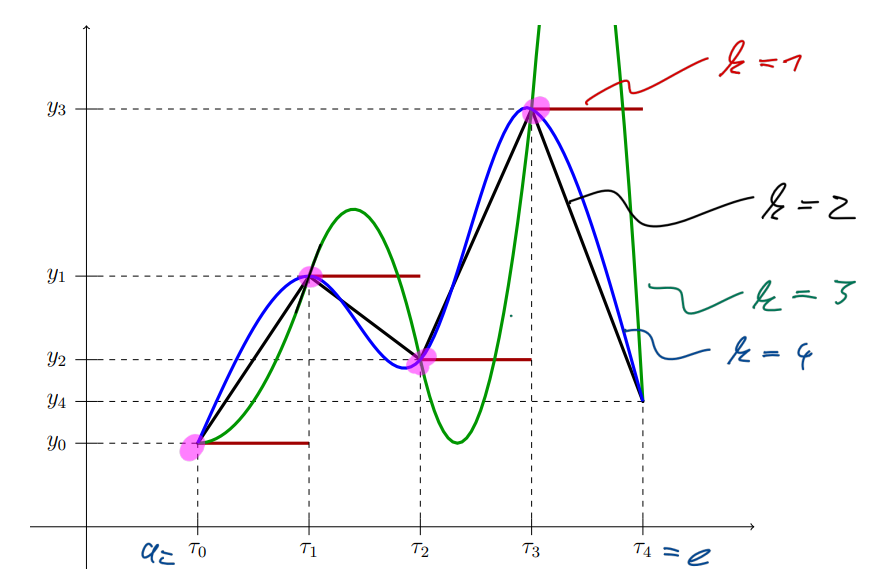
\includegraphics[scale=0.5]{assets/spline.png}
\end{center}


\subsubsection{Dimension Count (Degrees of Freedom)}
Without any smoothness constraints, a collection of unlinked piecewise polynomials of degree $k-1$ over $N$ intervals has a total dimension of:
$$\dim \Pi_{k-1,\tau} = k \cdot N$$

However, a spline space forces constraints at the internal boundaries. There are $N-1$ internal knots. At every single internal knot, the pieces must match exactly in value and in their first $k-2$ derivatives, which introduces $k-1$ smoothness conditions per internal knot. 

Every condition removes one free coefficient (degree of freedom). Therefore, the actual dimension of our smooth spline space is calculated by subtracting these constraints from our total unlinked pool:
\[\begin{aligned}
\dim \mathbb{P}_{k,\tau} &= \dim\Pi_{k-1,\tau} - (\text{internal knots}) \cdot (\text{conditions per knot}) \\
&= k N - (N-1)(k-1) \\
&= k N - (k N - k - N + 1) \\
&= k + N - 1
\end{aligned}\]

This final number, $k + N - 1$, tells us exactly how many data points/boundary conditions are needed to uniquely lock down and solve a complete spline function.
\subsubsection{Construction of Cubic Splines ($k=4$)}
From this point forward, we focus on the most widely used configuration: **cubic splines** ($k=4$). We aim to compute a piecewise cubic spline $s \in C^2([a, b])$. 

For each subinterval $i$ (where $0 \leq i < N$), the restriction of the spline to that interval is denoted as the individual polynomial piece:
\[s_i(x) := s(x)|_{[\tau_i, \tau_{i+1}]}\]

Each piece $s_i(x)$ is a polynomial of degree 3. If we hypothetically knew both the function values and the first derivatives at the endpoints of the subinterval:
\[y_i := s_i(\tau_i), \quad y_{i+1} := s_i(\tau_{i+1}) \quad \text{and} \quad y'_i := s'_i(\tau_i), \quad y'_{i+1} := s'_i(\tau_{i+1})\]
then finding $s_i(x)$ reduces to a standard **Hermite interpolation problem** on that localized interval. 

By defining the localized step size $h_i := \tau_{i+1} - \tau_i$ and a normalized local variable $t := \frac{x - \tau_i}{h_i}$ (where $t \in [0, 1]$), the localized cubic Hermite polynomial can be parameterized as:
\[s_i(x) = y_i + y'_i(x - \tau_i) + \left( \frac{y_{i+1} - y_i}{h_i^2} - \frac{y'_i}{h_i} \right)(x - \tau_i)^2 + \left( \frac{y'_{i+1} + y'_i}{h_i^2} - 2\frac{y_{i+1} - y_i}{h_i^3} \right)(x - \tau_i)^2(x - \tau_{i+1})\]

Grouping by our boundary variables yields the standard blending form:
\[s_i(x) = (1 - 3t^2 + 2t^3)y_i + (3t^2 - 2t^3)y_{i+1} + (t - 2t^2 + t^3)h_iy'_i + (t^3 - t^2)h_iy'_{i+1}\]

\paragraph{Why this formulation is chosen:} Because this local piece inherently uses the exact shared values $y_i, y_{i+1}$ and slopes $y'_i, y'_{i+1}$ at its boundaries, **the continuity of both the global function $s(x)$ ($C^0$) and its first derivative $s'(x)$ ($C^1$) is completely guaranteed by design.**

---

\subsubsection{Enforcing $C^2$ Continuity: Computing the Slopes}
When interpolating a given function $f(x)$, we immediately nail down our function values at the knots:
\[y_i = s(\tau_i) := f(\tau_i) \quad \text{for } 0 \leq i \leq N\]

Out of our total $N + k - 1 = N + 3$ degrees of freedom, fixing these $N+1$ values leaves exactly $(N+3) - (N+1) = 2$ free parameters left to determine. 

The core idea of spline construction is to use this remaining flexibility to **force the second derivatives to match smoothly at the inner knots**. We differentiate our blending equation $s_i(x)$ twice with respect to $x$:
\[s''_j(x) = (-6 + 12t)\frac{y_j}{h_j^2} + (6 - 12t)\frac{y_{j+1}}{h_j^2} + (-4 + 6t)\frac{y'_j}{h_j} + (-2 + 6t)\frac{y'_{j+1}}{h_j}\]

At every internal knot $\tau_i$ (for $0 < i < N$), the left-hand piece $s_{i-1}$ and the right-hand piece $s_i$ must share the exact same second derivative value:
\[s''_{i-1}(\tau_i) \overset{!}{=} s''_i(\tau_i)\]

Evaluating the derivatives at $t=1$ (for $s''_{i-1}$) and $t=0$ (for $s''_i$) and gathering the unknown slope parameters yields the continuity condition:
\[\frac{1}{h_{i-1}}y'_{i-1} + \left( \frac{2}{h_{i-1}} + \frac{2}{h_i} \right)y'_i + \frac{1}{h_i}y'_{i+1} = 3\frac{y_{i+1} - y_i}{h_i^2} + 3\frac{y_i - y_{i-1}}{h_{i-1}^2}\]

This equation provides $N - 1$ linear constraints. However, we have $N + 1$ unknown slope variables ($y'_0, y'_1, \dots, y'_N$) to solve for. We are missing exactly two equations.

---

\subsubsection{Boundary Conditions}
To close the linear system and uniquely fix our remaining 2 degrees of freedom, we must choose conditions at the outermost global boundaries of our domain, $a = \tau_0$ and $b = \tau_N$. Common choices include:

\begin{enumerate}
    \item \textbf{Natural Boundary Conditions:} We assume the spline flattens out entirely at the boundaries, meaning no curvature:
    \[s''(\tau_0) = s''(\tau_N) = 0\]
    \item \textbf{Periodic Boundary Conditions:} Useful if the target function is cyclic. We match the slopes and curvatures at both ends:
    \[y'_0 = y'_N \quad \text{and} \quad s''(\tau_0) = s''(\tau_N)\]
    \item \textbf{Clamped / Complete Boundary Conditions:} We explicitly prescribe the exact boundary velocities directly from known data:
    \[y'_0 = f'(a) \quad \text{and} \quad y'_N = f'(b) \quad (\text{often set directly to } 0)\]
\end{enumerate}

Choosing a boundary condition grants us the final 2 equations, bringing our total to $N+1$ linear equations for our $N+1$ unknown slopes $y'_i$.

---

\subsubsection{The Tridiagonal Linear System}
When combining the $N-1$ inner knot equations with boundary conditions (demonstrated here using a modified boundary scheme that incorporates the endpoint trends), the entire system maps beautifully into a highly sparse, structurally secure **Tridiagonal Matrix System**:

\[
\begin{pmatrix}
\frac{2}{h_0} & \frac{1}{h_0} & & & & \\
\frac{1}{h_0} & \frac{2}{h_0} + \frac{2}{h_1} & \frac{1}{h_1} & & & \\
& \frac{1}{h_1} & \frac{2}{h_1} + \frac{2}{h_2} & \frac{1}{h_2} & & \\
& & \ddots & \ddots & \ddots & \\
& & & \frac{1}{h_N-2} & \frac{2}{h_{N-2}} + \frac{2}{h_{N-1}} & \frac{1}{h_{N-1}} \\
& & & & \frac{1}{h_{N-1}} & \frac{2}{h_{N-1}}
\end{pmatrix}
\begin{pmatrix}
y'_0 \\
y'_1 \\
y'_2 \\
\vdots \\
y'_{N-1} \\
y'_N
\end{pmatrix}
=
\begin{pmatrix}
3\frac{y_1 - y_0}{h_0^2} \\
3\frac{y_1 - y_0}{h_0^2} + 3\frac{y_2 - y_1}{h_1^2} \\
3\frac{y_2 - y_1}{h_1^2} + 3\frac{y_3 - y_2}{h_2^2} \\
\vdots \\
3\frac{y_{N-1} - y_{N-2}}{h_{N-2}^2} + 3\frac{y_N - y_{N-1}}{h_{N-1}^2} \\
3\frac{y_N - y_{N-1}}{h_{N-1}^2}
\end{pmatrix}
\]

Because this system matrix is strictly diagonally dominant, it is guaranteed to be invertible, confirming that a unique cubic spline solution **always exists** and is **stable**.

---

\subsubsection{Computational Complexity, Error, and Conditioning}

\paragraph{Computational Effort:}
\begin{itemize}
    \item \textbf{Solving the Tridiagonal System:} Because the system is tridiagonal, we don't need expensive Gaussian elimination ($\mathcal{O}(N^3)$). Instead, we apply the specialized **Thomas Algorithm** (Tridiagonal Matrix Algorithm), which solves for all slopes in **$\mathcal{O}(N)$ linear execution time**.
    \item \textbf{Evaluating the Spline Pieces:} Once the slopes $y'_i$ are cached, setting up the $N$ individual pieces $s_i(x)$ scales linearly as **$\mathcal{O}(N)$**. Local evaluation of a value $x$ requires finding the matching interval via binary search ($\mathcal{O}(\log N)$) followed by a fast evaluation of the localized polynomial.
\end{itemize}

\paragraph{Approximation Error (Cubic Splines):}
Assuming our target function is sufficiently smooth ($f \in C^4([a,b]$)), let $h = \max_{i} h_i$ represent the largest interval width in our partition. The global approximation error decreases rapidly as we refine the mesh:
\[\|f - s\|_{\infty} \leq C \cdot h^4 \|f^{(4)}\|_{\infty}\]
This indicates an optimal **fourth-order convergence rate** $\mathcal{O}(h^4)$. Refining the grid by dividing the subinterval spacing in half reduces the global error by a factor of $16$.

\paragraph{Conditioning and Stability Analysis:}
Global polynomial interpolation on equidistant nodes suffers severely from poor conditioning and wild edge oscillations (Runge's Phenomenon), causing the Lebesgue constant to grow exponentially. 

In stark contrast, **piecewise splines exhibit outstanding numerical conditioning stability**. Because the calculation matrix is strictly diagonally dominant, localized measurement perturbations or floating-point rounding errors injected at a specific data knot $y_i$ decay exponentially as they travel away from the source. The system remains bounded and reliable regardless of how large $N$ grows.

\subsection{Trigonometrical Interpolation}
Note: The polynomial interpolation will be done in $\mathbb{C}$. We are given a set of support points, and tasked to compute the coefficients of the polynomial that interpolates those points.

We are interpretating the interpolated Polynomial with $\cos$ and $\sin$. This is the \textbf{Fourier Transform}.

So we get a super fast algorithm to solve this interpolation problem \textbf{Fast Fourier Transform} $\mathcal{O}(n\log n)$.

\subsubsection{Reminder of Complex Numbers}
\[z_1 := a_1 + b_1 i = r_1e^{i\phi_1}\]
\[z_2 := a_2 + b_2 i = r_2e^{i\phi_2}\]
Just remember that in polar form operations are slightly different given we are working with exponentiation.

\subsubsection{Support points and interpolated polynomial}
We have the complex $n$-th Identity root $\omega_n := e^{2\pi i /n}$.

The support points $z_j := \omega_n^{j} , \ 0 \leq j \leq n-1$ which are equidistant on the identity circle.

The support values $v_j \in \mathbb{C}, \ 0 \leq j \leq n-1$.

The Lagrange-Interpolation polynomial: $P_{n-1}(z) = \sum_{k=0}^{n-1}c_kz^k$ with $P_{n-1}(z_j) = \sum_{k=0}^{n-1} c_kz_j^k = \sum_{k=0}^{n-1}c_k\omega_n^{j\cdot k} = v_j$.

$c$ for coefficient, $v$ for value.

\paragraph{Discrete Fourier Transform (DFT)}: It's a function from the 'values' (or support points) to the coefficients:
\[\vec{v} := (v_j)_{0\leq j\leq n-1} \longrightarrow \vec{c} := (c_k)_{0\leq k \leq n-1}\]
The inverse is called Inverse Discrete Fourier Transform (IDFT) and stupidly, it maps from the coefficients to the support points (so it's just writing the support points in the function and getting the support values back).

\subsubsection{Interpretation of $P_{n-1}$ as a periodical function $\mathbb{R}\to\mathbb{C}$}
If we look at the mapping $z : \mathbb{R}\to\mathbb{C}$:
\[t\to z(t) := e^{2\pi i t} = \cos(2\pi t) + i\sin(2\pi t)\]
The function cycles around the unity circle. The full circle is in the range $[0,1]$ but it keeps cycling.

Then $z(t)^k = e^{2\pi i k t} = \cos(2\pi k t) + i \sin(2\pi k t)$.

And then:
\[p(t) := P_{n-1}(z(t)) = \sum_{k=0}^{n-1}c_k(\cos(2\pi k t) + i \sin(2\pi kt))\]
and if we set $t_j = j/n$:
\[p(t_j) = \sum_{k=0}^{n-1}c_k(\cos(2\pi k j/n) + i\sin(2\pi kj/n))\]
And this view explains the polynomial interpolation.

\paragraph{Interpolation matrix $M$}: With the interpolation matrix 
\[M := (z_j^k)_{0\leq j,k \leq n-1} = ((\omega_n^j)^k)_{0\leq j,k\leq n-1} = (\omega_n^{jk})_{0\leq j,k \leq n-1}\]
Which is the \textbf{Vandermonde} matrix. Which represents the $k$-th power of the $j$-th support point.

So the IDFT:
\[v_j = \sum_{k=0}^{n-1}c_kz_j^k = \sum_{k=0}^{n-1}c_k\omega_n^{jk}\]
so $\vec{v} = M \vec{c}$.

\textbf{Interesting}: The following is true:
\[M^{-1} = \frac{1}{n}\overline{M} = \frac{1}{n}(\omega_n^{-j\cdot k})_{0\leq j,k \leq n-1}\]
\textbf{Proof}: If we write out the $k$-th row of $\frac{1}{n}\overline{M}\vec{v}$:
\[\frac{1}{n}\sum_{j=0}^{n-1}v_j\omega_n^{-jk} = \frac{1}{n}\sum_{j=0}^{n-1}\left(\sum_{l=0}^{n-1}c_l\omega_n^{jl}\right)\omega_n^{-jk}\]
\[ = \frac{1}{n}\sum_{j=0}^{n-1}\sum_{l=0}^{n-1}c_l \omega_n^{j(l-k)} = \frac{1}{n}\sum_{l=0}^{n-1}c_l\sum_{j=0}^{n-1}\left(\omega^{l-k}_n\right)^j\]
We set $q := \omega_n^{l-k}$. And we know because of the geometric series $\sum_{j=0}^{n-1}q^j = \frac{q^n-1}{q-1}$ for $q\neq 1$. And because $q = \omega_n^{l-k} = 1 \iff l-k \equiv 0 \pmod n \iff l-k = 0$.

So if $l\neq k$:
\[\sum_{j=0}^{n-1}(\omega_n^{l-k})^j = \frac{\omega_n^{(l-k)\cdot n} - 1}{\omega_n^{l-k} - 1} = 0\]
If $l = k$:
\[\sum_{j=0}^{n-1}1 = n\]
So knowing this:
\[ = \frac{1}{n}\sum_{l=0}^{n-1}c_l\sum_{j=0}^{n-1}(\omega_n^{l-k})^j = \frac{1}{n}(n\cdot c_k) = c_k\]
So we have proven that when computing the $k$-th row we get the $k$-th coefficient. Because we have, our equality is true.

So knowing this, we can compute the DFT as:
\[\vec{c} = \frac{1}{n}\overline{M}\vec{v} = \frac{1}{n}\overline{M\bar{\vec{v}}}\]

\subsubsection{Fast Fourier Transform (FFT)}
\paragraph{Idea}: From now on, $n = 2^p$ with $p > 0$, we can compute $\text{IDFT}(\vec{c})$ in $\mathcal{O}(n\log n)$ operations. We use divide and conquer. We split at halfpoint $m := n/2$.

First half of coefficients $0 \leq j < m$:
\[v_j = \sum_{k=0}^{n-1}c_k\omega_n^{jk} = \sum_{k=0}^{m-1}c_{2k}\omega_n^{2kj} + \sum_{k=0}^{m-1}c_{2k+1}\omega_n^{(2k + 1)j}\]
We have split into even and odd coefficients. Below we can notice that $\omega_n^{2k} = \omega_m^k$:
\[= \sum_{k=0}^{m-1}c_{2k}\omega_m^{kj} + \omega_n^j\sum_{k=0}^{m-1}c_{2k+1}\omega_m^{kj}\]
And we just do a recursive call for each of the two components. The issue is that this strategy is not that efficient, we do four recursive calls (two for each half), so we aren't really winning anything. The key is that we can use the same two calls from the first half for the second half.

Second half, $0 \leq j < m$:
\[v_{m+j} = \sum_{k=0}^{n-1}c_k\omega_n^{(m+j)k} = \sum_{k=0}^{m-1}c_{2k}\omega_n^{2k(m+j)} + \sum_{k=0}^{m-1}c_{2k+1} \omega_n^{(2k+1)(m+j)}\]
And because $\omega_n^{2km}= \omega_n^{kn} = 1$:
\[ = \sum_{k=0}^{m-1}c_{2k}\omega_m^{kj} - \omega_n^j\sum_{k=0}^{m-1}c_{2k+1}\omega_m^{kj}\]
So for each level, we do two recursive calls on $T(n/2)$ and a linear time complexity on each call.

So in total:
\[T(n) = 2T(n/2) + \Theta(n) \in \Theta(n\log n)\]

This implementation of the IDFT is called the Fast Inverse Fourier Transform.

\section{Quadrature}
Roughly translates to 'finding the area of'.

\subsection{Problem Setting}
We are going to be looking at $f \in C^0([a,b])$ (with the exponent referring to how often the function can be continuously differentiable).

Our goal is to compute:
\[I(f):= \int_a^b f(x) \, dx\]
$I$ is a linear mapping $C^0([a,b]) \to \mathbb{R}$, which makes it a \textbf{linear functional}.

And we can trivially see that for $f,g \in C^0([a,b])$ and $\alpha,\beta \in \mathbb{R}$:
\[I(\alpha f + \beta g) = \alpha I(f) + \beta I(g)\]

The idea is to approximate $I$ as a linear combination of evaluation functionals $\mu_{\text{aus},x^*}: g \to g(x^*)$:
\[I(f) \approx \tilde{I}(f) = (b-a)\sum_{j=0}^m c_j f(x_j)\]

The evaluation points $x_j$ and weights $c_j$ for $0 \leq j \leq m$ define a \textbf{Quadrature rule}.

\begin{center}
  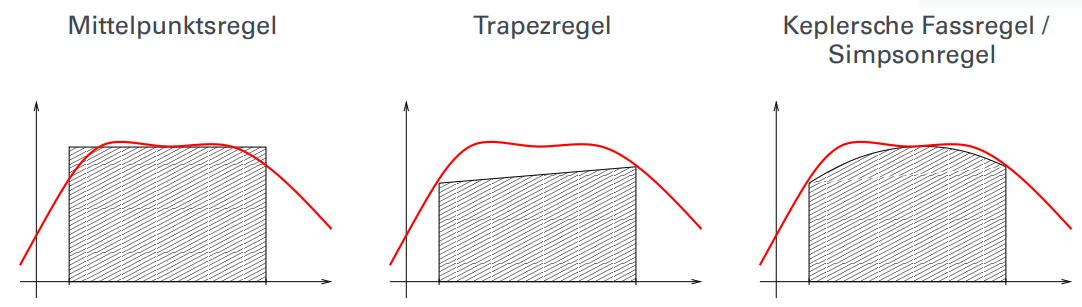
\includegraphics[scale=0.5]{assets/quadrature_rules.png}
  \begin{itemize}
    \item \textbf{Middle point rule:} $m=0$, $x_0 = \frac{a+b}{2}$, $c_0 = 1$
    \item \textbf{Trapezoidal rule:} $m = 1$, $x_0 = a, \ x_1 = b$, $c_0 = \frac{1}{2}, \ c_1 = \frac{1}{2}$
    \item \textbf{Simpson's rule:} $m = 2$, $x_0 = a, \ x_1 = \frac{a+b}{2}, \ x_2 = b$, $c_0 = c_2 = \frac{1}{6}, \ c_1 = \frac{2}{3}$
    
    \[\tilde{I}(f) = \frac{b-a}{6}\left(f(a) + 4f\left(\frac{a+b}{2}\right) + f(b)\right)\]
  \end{itemize}
\end{center}



\subsection{Interpolation}
We want to approximate $f$ through an interpolating function $\tilde{f}$:
\[\tilde{I}(f) := I(\tilde{f}) = \int_a^b \tilde{f}(x) \, dx\]

So the Quadrature error can be bounded as:
\[
\begin{split}
|I(f) - \tilde{I}(f)| &= \left|\int_a^b f(x) \, dx - \int_a^b \tilde{f}(x) \, dx\right| \\
&\underbrace{=}_{\text{linearity}} \left|\int_a^b (f(x) - \tilde{f}(x)) \, dx\right| \\
&\leq \int_a^b |f(x) - \tilde{f}(x)| \, dx \\
&\leq \int_a^b \max_{x\in [a,b]} \underbrace{|f(x) - \tilde{f}(x)|}_{=: \|f-\tilde{f}\|_\infty} \, dx = (b-a)\|f-\tilde{f}\|_\infty
\end{split}
\]
Which is bounded by the maximum \textbf{interpolation error}.

\subsection{Degree of Accuracy}
A Quadrature rule $\tilde{I} \approx I$ has a degree of accuracy $k \in \mathbb{N}_0$ if $k$ is the maximal value such that:
\[\forall Q \in \Pi_k : \tilde{I}(Q) = I(Q)\]
In plain terms: 'How complex of a polynomial can this Quadrature rule integrate flawlessly?'

A degree of accuracy $= 0$ means it can integrate constant functions perfectly (almost all rules satisfy this). The condition for it is:
\[\forall \alpha \in \mathbb{R}: \tilde{I}(x \to \alpha) = I(x \to \alpha) = \alpha(b-a)\]
Because of linearity, it is enough to prove it for $\alpha = 1$, since $I(x \to \alpha) = \alpha I(x \to 1)$.

\subsection{Procedural Error Example in Trapezoidal Rule}
Let $\tilde{f} = P(f \mid a,b)$ be the linear interpolant. Using Taylor's remainder formula for polynomial interpolation ($m=1$):
\[f(x) - \tilde{f}(x) = \frac{f^{(m+1)}(\xi(x))}{(m+1)!}\Phi_m(x) = \frac{1}{2}(x-a)(x-b)f''(\xi(x))\]

So the exact procedural error expression is:
\[I(f) - \tilde{I}(f) = \int_a^b (f(x) - \tilde{f}(x)) \, dx = \frac{1}{2}\int_a^b (x-a)(x-b)f''(\xi(x)) \, dx\]

Since the term $(x-a)(x-b) \leq 0$ does not change its sign for any $x \in [a,b]$, we can apply the \textbf{Generalized Mean Value Theorem for Integrals}. This lets us pull the second derivative out of the integral at an intermediate point $\zeta \in [a,b]$:
\[I(f) - \tilde{I}(f) = \frac{1}{2} f''(\zeta) \int_a^b (x-a)(x-b) \, dx\]

Evaluating the remaining polynomial integral yields $\int_a^b (x-a)(x-b) \, dx = -\frac{1}{6}(b-a)^3$. Substituting this back in gives the finalized procedural error:
\[I(f) - \tilde{I}(f) = -\frac{1}{12}(b-a)^3 f''(\zeta)\]

\subsection{Newton-Cotes Formulas}
\subsubsection{Quadrature Through Polynomic Interpolation}
We approximate $f$ through the polynomial $\tilde{f} = P(f \mid x_0,\dots,x_m)$, and define $I_m(f) := I(\tilde{f})$.
This rule $I_m$ has a degree of accuracy of at least $m$:
\[Q \in \Pi_m \implies \tilde{f} = Q \implies I_m(Q) = I(\tilde{f}) = I(Q)\]

We will structure this into the following standard component form ('Baukasten-Form'):
\[I_m(f) = (b-a) \sum_{j=0}^m c_j f(x_j)\]

If we write out the Lagrange representation of the polynomial:
\[P(f \mid x_0,\dots,x_m) = \sum_{j=0}^m f(x_j) l_{j,m}(x)\]
Then, leveraging the linearity of integrals:
\[I_m(f) = \int_a^b \sum_{j=0}^m f(x_j) l_{j,m}(x) \, dx = \sum_{j=0}^m f(x_j) \underbrace{\int_a^b l_{j,m}(x) \, dx}_{= \tilde{c}_j = c_j \cdot (b-a)}\]

Since $l_{j,m} \in \Pi_m$, a quadrature rule with a degree of accuracy of at least $m$ must integrate it perfectly. Therefore, for each $0 \leq j \leq m$:
\[\underbrace{\int_a^b l_{j,m}(x) \, dx}_{I(l_{j,m})} = \underbrace{(b-a)\sum_{i=0}^m c_i l_{j,m}(x_i)}_{\tilde{I}(l_{j,m})} = (b-a)c_j\]

From this, we conclude that the weights can be calculated explicitly via:
\[c_j = \frac{1}{b-a}\int_a^b l_{j,m}(x) \, dx\]
This provides a direct way to compute the weights $c_j$.

Consequently, this confirms that for any $f \in \Pi_m$:
\[\tilde{I}(f) = (b-a)\sum_{j=0}^m \left(\frac{1}{b-a}\int_a^b l_{j,m}(x) \, dx\right) f(x_j) = \int_a^b \sum_{j=0}^m f(x_j) l_{j,m}(x) \, dx = \int_a^b f(x) \, dx\]
This formally verifies the degree of accuracy.

\subsubsection{Newton-Cotes Formula}
If we distribute the support points equidistantly over the interval $[a,b]$:
\[x_j = a + (b-a)\frac{j}{m} \quad 0 \leq j \leq m\]
And compute the weights $c_j$ as derived above, we obtain the standard Newton-Cotes formulas.

\begin{center}
  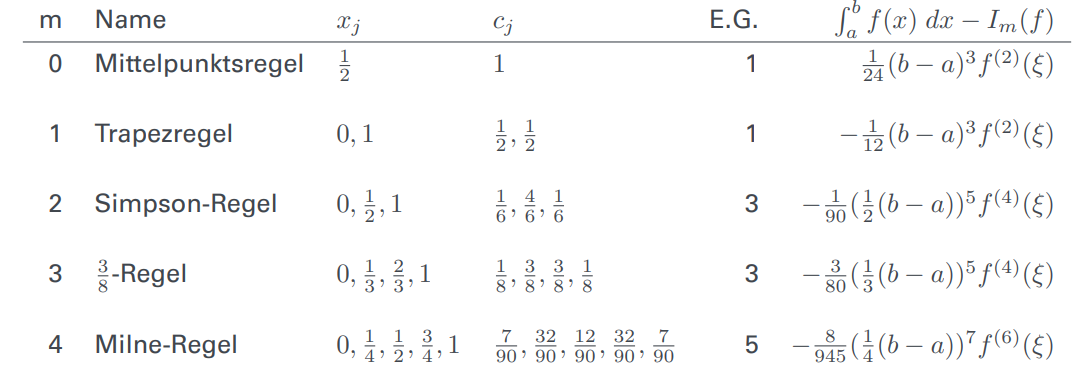
\includegraphics[scale=0.5]{assets/newton_cotes.png}
\end{center}
The drawback is that for high orders ($m \geq 8$), the weights $c_j$ can become negative, which causes numerical instability.

\subsection{Clenshaw-Curtis Quadrature}
The alternative idea is to distribute the support points using the roots/extrema of the Chebyshev polynomials:
\[x_j = \frac{a+b}{2} - \frac{b-a}{2}\cos\left(\frac{\pi}{m}j\right)\]

\begin{center}
  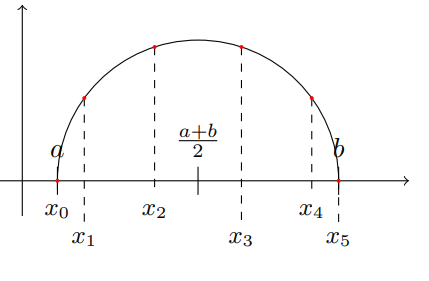
\includegraphics[scale=0.5]{assets/clenshaw_curtis_quadrature.png}
\end{center}
By clustering the points closer to the boundaries of the interval, we preserve strictly positive weights $c_j$ even for large values of $m$, avoiding the stability issues of Newton-Cotes.



\subsection{Gaussian Quadrature}
We want to hunt the Quadrature rule with the maximal degree of accuracy

\subsubsection{Motivation}
If we pick the weights $c_0,...,c_m$ so that

\[\text{Degree of accuracy at least }m \Leftrightarrow c_j = (b-a)\int_a^b l_{j,m}(x)dx\]
m+1 further degrees of freedom $x_0,...,x_m$ (which are the support points)

Is it even possible to reach a degree of accuracy of $2m +1 $? Maybe even more?


\textbf{YES!:} The middle-point rule gave us for $m = 0$ , $2m+1 = 1$! Can we also make this happen for the Simpson rule?

\paragraph{How far can we push the degree of accuracy?} For no pick of $x_0,...,x_m$ can we get degree of accuracy of $2m+2$ or more.

To prove this, we are given $x_0,...,x_m$ and we are looking for a $Q\in \Pi_{2m+2}$ that cannot be exactly integrated. The strategy to easily prove this is build a polynomial so that the integral is $\neq 0$ but the approximation gives us $=0$

To do this, we build a polynomial that for all $m+1$ support points, its value is zero.
\[Q(x) =  \Pi_{j=0}^m(x-x_j) = \phi_m(x) \in \Pi_{m+1}\]

\[\tilde{I}(Q) = (b-a)\sum_{j=0}^mc_j\underbrace{Q(x_j)}_{=0} = 0\]
So now we have guaranteed that the approximation is zero, but we don't know the value of the true integral. So we do a little switch and quadrate the function
\[Q(x) = \phi_m^2(x) \in \Pi_{2m+2}\]
The approximation is still zero, but the true integral.

\[I(Q) = \int_a^b Q(x)dx\]
This true integral is greater than zero because $\phi^2(x) \geq 0 \quad \forall x$, and because the function is non-zero (finite many zero evaluations), the total integral cannot be zero.

We have an upper bound, what about the actual maximum value we can reach? 
\paragraph{Ceiling: } There is exactly one set of support points $x_0,...,x_m$ so that the quadrature rule gets a degree of accuracy of $2m+1$. The zeroes of the \textbf{Lagrange Polynomial}

\subsubsection{Scalar Product and Orthogonality}
\label{subsubsec:scalar_prod_orthogonality}
For the construction is the principle of orthogonality pretty important. We are talking here regarding the space of all polynomials $\Pi$, we call the $L^2$-Scalar product
\[\langle f,g \rangle := \int_{-1}^1 f(x)g(x)dx\]
So polynomials p,q are orthogonal if $\langle p,q \rangle = 0$

Some examples below ($x$ means $x\to x$ and so on )
\[\langle x,x \rangle = \int_{-1}^1 x^2 dx = \frac{2}{3}\]
\[\langle x^3, x \rangle \int_{-1}^1 x^4 dx = \frac{2}{5}\]
And if we define $p(x) := x^3 - \underbrace{\frac{\langle x^3 , x\rangle}{\langle x,x \rangle}}_{=3/5}x$ then
\[\langle p , x \rangle = \langle x^3, x\rangle - \frac{\langle x^3 , x \rangle}{\langle x,x \rangle} \langle x,x \rangle = 0\]

\subsubsection{Legrende Polynomials}
It's an orthogonal basis of polynomials.

$\tilde{P}_0(x) := 1$

And for $n > 1$, $x^n$ orthogonalisieren.
\[\tilde{P}_n(x) := x^n - \sum_{i=0}^{n-1}\frac{\langle \tilde{P}_i, x^n\rangle}{\langle \tilde{P}_i, \tilde{P}_i\rangle} \tilde{P}_i(x)\]

Polynomials $\tilde{P}_n$ with degree n and leading coefficient 1, orthogonal to all polynomials of a smaller degree.
\[\langle\tilde{P}_n, p  \rangle \int_{-1}^1 \tilde{P}_n(x) p(x)dx = 0 \quad \forall p \in \Pi_{n-1}\]

And we define the Legrende polynomials as
\[P_n(x) = \frac{\tilde{P}_n(x)}{\tilde{P}_n(1)} \quad \text{Normalizing so that }P_n(1) = 1\]

And an easier to remember recursive formula for the Legrende polynomials
\[P_0(x)= 1, P_1(x) = x , P_n(x) = \frac{2n-1}{n}xP_{n-1}(x) - \frac{n-1}{n}P_{n-2}(x) \quad n \geq 2\]

\begin{center}
  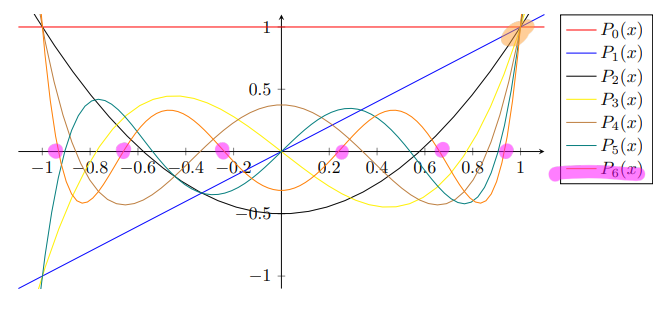
\includegraphics[scale=0.5]{assets/legrende_polynomials.png}
\end{center}

\paragraph{Extra:} We can prove that $P_n$ has $n$ zeroes in $[-1,1]$

\paragraph{Proof of Ceiling:}
Proof idea(not for zeroes, but for the Ceiling, mentioned above \hyperref[subsubsec:scalar_prod_orthogonality]{Scalar Product and Orthogonality} ): Support points $x_0,...,x_m$ zeroes of $\tilde{P}_{m+1}(x) = (x-x_0)(x-x_1)...(x-x_m)$

We want to prove that $\forall p \in \Pi_{2m+1}$ is exactly integrated by $\tilde{I}$

\[p(x) - \sum_{j=0}^m p(x_j)l_{j,m}(x) \quad \text{ has at least zeroes }x_0,x_1,...,x_m\]
So we can split it into 
\[p(x) - \sum_{j=0}^m p(x_j)l_{j,m}(x) = q(x)\underbrace{(x-x_0)(x-x_1)...(x-x_m)}_{\tilde{P}_{m+1}(x)} \quad q(x) \in \Pi_m\]

Integrate
\[\underbrace{\int_{-1}^m p(x)dx}_{I(p)} - \underbrace{\sum_{j=0}^m p(x_j)\int_{-1}^1l_{j-m}(x)dx}_{\tilde{I}(p)} = \int_{-1}^1 q(x)\tilde{P}_{m+1}(x)dx = 0\]
We just proved that the integration is exact

\paragraph{Proof Pt.2 (opposite direction) }: Let $x_0,...,x_m$ be, so that all $p \in \Pi_{2m+1}$ is exactly integrated by $\tilde{I}$. We want to prove that $\phi_m = (x-x_0)...(x-x_m)$ is orthogonal to all $q\in\Pi_m$

Following this, $\phi_m = cP_n(x)$, and because Leading coefficient 1, $\phi_m = \tilde{P}_{m+1}$

So we know that 
\[q(x)\phi_m(x) \in \Pi_{2m+1}\]
Integration is easy because of the degree of accuracy
\[\int_{-1}^1 q(x)\phi_m(x)dx = \underbrace{2}_{(b-a) = (1+1)}\sum_{j=0}^m c_j q(x_j) \cdot \underbrace{\prod_{i=0}^m \left(x_j - x_i\right)}_{=0} = 0\]

\subsubsection{The weights $c_j$ of the Gaussian Quadrature are positive}
For $0 \leq i \leq m$
\[l_{i,m}(x) \in \Pi_m \quad so \, \l_{i,m}^2(x)\in \Pi_{2m} \subseteq \Pi_{2m+1}\]
So then, $l_{i,m}^2$ can be exactly integrated.
\[0 < \int_{-1}^1 l_{i,m}^2  = \tilde{I}(l_{i,m}^2) = 2\sum_{j=0}^m c_jl_{i,m}^2(x_j)\]
And because we know
\[l_{i,m}(x_j) \begin{cases}
  1 \quad i=j\\
  0 \quad i \neq j
\end{cases} = l_{i,m}^2(x_j)\]
So quadration is irrelevant so we can strip it
\[\int_{-1}^1 l_{i,m}^2= 2\sum_{j=0}^m c_jl_{i,m}(x_j) = 2c_i\]
So this concludes that all the weights are positive.

\subsection{Composite Quadrature Formulas}
The rough idea is paritioning the integration interval into subintervals.

\subsubsection{Construction}
Error trapezoid rule
\[E_1(f) := I(f) - I_1(f) = - \frac{1}{12}(b-a)^3f''(\xi)\]
We can split it into separate polynomials
\[a = \tau_0 < \tau_1 < ... <\tau_N = b\]
The separation is equidistant $h:= (b-a)/N$, and $\tau_i = a+ih$

So on each subinterval the Quadrature rule $\tilde{I}$ with error $E(f|_{[\tau_i,\tau_{i+1}]}) \in O(h^\alpha) = O(N^{-\alpha})$. If we sum it up the total error
\[I(f) - \sum_{i=0}^{N-1}\tilde{I}(f|_{[\tau_i,\tau_{i+1}]}) = \sum_{i=0}^{N-1}E(f|_{[\tau_i,\tau_{i+1}]}) \in O(N^{-\alpha + 1})\]

\subsubsection{Trapezoid sum}
\begin{center}
  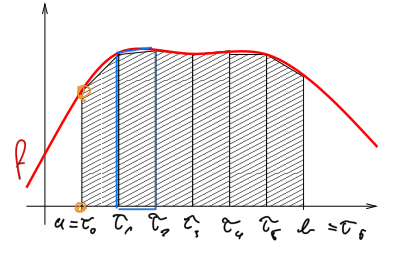
\includegraphics[scale=0.5]{assets/trapezoid_sum.png}
\end{center}

\[T(h) = h\sum_{i=0}^{N-1}\frac{f(\tau_i) + f(\tau_{i+1})}{2} = \]
\[ = h\left[\frac{f(\tau_0)}{2} + \sum_{i=1}^{N-1}f(\tau_i) + \frac{f(\tau_{N})}{2}\right]\]
\[ = (b-a)\sum_{j=0}^N c_jf(x_j)\]
And with $x_j = \tau_j$, then $\underbrace{c_0 = c_N = \frac{1}{2N}, \, c_j = \frac{1}{N}}_{\geq 0, \sum c_j = 1}$

\begin{itemize}
  \item Costs: $N+1$ evaluations
  \item Error:
  \[\sum_{i=0}^{N-1}(-\frac{1}{12}h^3 f''(\xi)) \underbrace{=}_{\text{no proof}} \frac{1}{12}h^3 N f''(\xi) = -(b-a)h^2 \frac{f''(\xi)}{12} \]
  \item Degree of accuracy: $1$
\end{itemize}
\subsubsection{Simpson Sum}
\[S(h) = \frac{h}{6} \left[ f(\tau_0) + 4 f(\frac{\tau_0 + \tau_1}{2}) + 2f(\tau_1) + 4... + 2... + ... + f(\tau_N)\right]\]

\begin{itemize}
  \item Costs: $2N+1$ evaluations
  \item Error:
  \[\frac{-1}{90\cdot 2^5}h^5 f^{(4)}(\xi) \frac{b-a}{h} \in O(h^4)\]
  \item Degree of accuracy: $3$
\end{itemize}

\paragraph{Side by side comparison}
\begin{center}
  \begin{tabular}{|c|c|c|}
    \hline
     & $T(h)$ & $S(h)$ \\
     \hline
     Costs & $O(N)$ & $O(N)$ \\
     \hline
     Error & $O(N^{-2})$ & $O(N^{-4})$ \\
    \hline
    Assumption & $f\in C^2$ & $f\in C^4$ \\
    \hline
  \end{tabular}
  
  So stricter assumptions, but same cost and less error and higher degree of accuracy.
\end{center}
\subsection{Uselessness of Simpson Sum}
We are able to compute $S(h)$ with $T(h)$ and $T(h/2)$

\begin{itemize}
  \item $T(h)$ has the same support points as usual
  \item $T(h/2)$ has double as many support points
\end{itemize}
This is the table of weights assigned at each $\tau$ (spacing between $\tau$ is still $h$)
\begin{center}
  \begin{tabular}{|c|c|c|c|c|}
    \hline
     & $\tau_0$ & $\frac{\tau_0 + \tau_1}{2}$ & $\tau_1$ & Nomenclature\\
    \hline
    $T(h)$ & $h/2$ & 0 & $h$ & $c_{T,h,j}$\\
    \hline
    $T(h/2)$ & $h/4$ & $h/2$ & $h/2$ & $c_{T,h/2,j}$ \\
    \hline
    $S(h)$ & $h/6$ & $4h/6$ & $2h/6$ & $c_{S,h,j}$\\
    \hline
  \end{tabular}
\end{center}
So each support point $x_j$ has the weights $c_{T,h,j}$, $c_{T,h/2,j}$, $c_{S,h,j}$.

And we can notice that
\[c_{S,h,j} = \frac{4}{3}c_ {T,h/2,j} - \frac{1}{3}c_{T,h,j}\]


So we can conclude that
\[S(h) = \frac{4}{3}T(h/2) - \frac{1}{3}T(h)\]
\paragraph{Error rate}: We know from the table that $T(h)$ had an error of $O(h^2) = O(N^{-2})$.

This means that
\[T(h)-I(f) = c_1 h^2 + \dots\]
which means
\[T(h/2) - I(f) = c_1 \left(\frac{h}{2}\right)^2 + \dots\]
And if we compute the total error
\[\frac{4}{3}\left(T(h/2) - I(f)\right) - \frac{1}{3}\left(T(h) - I(f)\right) = \]
\[\frac{4}{3}\left(c_1 \frac{h^2}{4}+ ...\right) - \frac{1}{3}\left(c_1h^2 + \dots\right) = 0\cdot h_1 + \dots\]
So the leading term ($h^2$) is zero, and eliminated!

\[\frac{4}{3}\left(T(h/2) - I(f)\right) - \frac{1}{3}\left(T(h) - I(f)\right) = \]
\[\left(\frac{4}{3}T(h/2) - \frac{1}{3}T(h)\right) - I(f) = S(h) - I(f) \in O(h^4)\]
And we are able to see the next term in the error, and it is $h^4$! Just by operating with two $h^2$ functions we were able to reduce the error up to $h^4$

\paragraph{Euler-Maclaurin Formula}: It's a formula that reveals the structure of the error rate of the trapezoid sum. For a $f \in C^{2p+2}$ there are $c_1,...,c_p$ (independent from f, independent from h) so that
\[T(h) - I(f) = c_1h^2 + c_2h^4 + c_3h^6 + ...+c_ph^{2p} + O(h^{2p+2})\]

And using this we are able to compute a 'Turbo' for the trapezoid sum
\paragraph{Turbo Trapezoid Sum}: 
\begin{enumerate}
  \item For $p+1$ different grid widths $h_i$ we compute the trapezoid sum
  \[\text{Example: }h_i := 2^{-i}h \quad 0 \leq i < p\]
  \item For each $T(h_i)$, write out the Euler-Maclaurin Formula. We set up a System of Linear Equations with $p+1$ equations and $c_1,...,c_p$ unknowns.
  \item Shape it into an upper triangle with the usual operations of
  \[row_i = \alpha\cdot row_i - \beta\cdot row_j \quad : \quad \alpha - \beta = 1\]
  \item Now on the left side of the last row of the System there is
  \begin{itemize}
    \item A linear expression in the $T(h_k)$: That is our approximation $T_p(h)$ of the integral
    \item Minus $I(h)$ (this is because we forced $\alpha-\beta = 1$)
  \end{itemize}
  \item And on the right side of the last row we have $O(h^{2p+2})$
\end{enumerate}
So we just made an algorithm with extremely high error order $h^{2p+2}$! The rough intuition is that we are able to eliminate error terms by repeating what we found out for the Simpson sum based on the trapezoid sum.

\subsubsection{Alternative (better) Perspective: Extrapolation}
Build $T(h) - I(f)$ as a function of $h$

Determine the interpolating polynomial $P_p$ with $P_p(h_i) = T(h_i) \quad 0 \leq i < p$

And we can compute $P_p(0)$ as a substitution for $\lim_{h\to 0}T(h)$ (so we interpolate the polynomial that for a given grid width gives us the integral, and then we get the value at grid width $=0$)

\begin{center}
  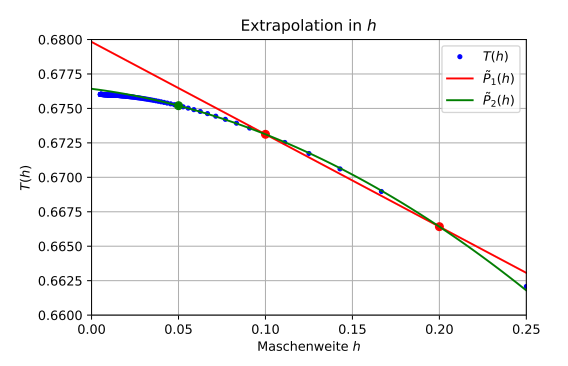
\includegraphics[scale=0.5]{assets/extrapolation.png}

  \begin{itemize}
    \item   The true value of the integral is $I(f) = 0.676$
    \item We can see that for $T(h)$, the wider the grid width, the worse the estimate is. 
    \item The first interpolation $P_1(h)$ interpolates only based on the values $T(h_1)$ and $T(h_2)$. Not too good of a result
    \item $P_2(h)$ gives us a basically perfect approximation, and we can get the actual value at $h=0$. Trying to compute for $h\approx 0$ with $T(h)$ would be computationally infinite, so we use the interpolation.
  \end{itemize}
\end{center}

\paragraph{Complication: We extrapolate better in $h^2$ than in $h$}: If we look at the Euler-Maclaurin Formula and we set $\xi := h^2$
\[T(h) = I(f) + \sum_{j=1}^p c_j h^{2j} + O(h^{2p+2}) = I(f) + \sum_{j=1}^pc_j \xi^j + O(h^{2p+2})\]

\begin{center}
  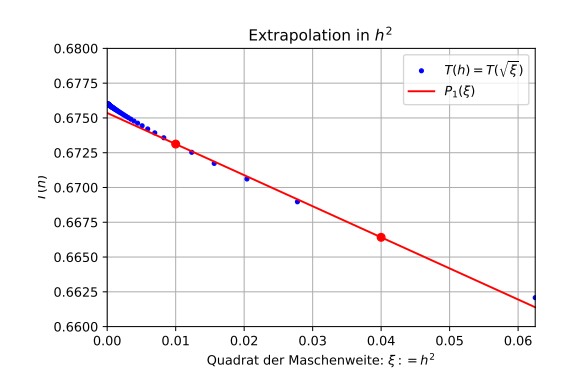
\includegraphics[scale=0.5]{assets/extrapolation_2.png}

  Same exact example as before (different axis for graph). But we can see, $P_1(h)$ is already much, much better.
\end{center}
We compute
\[T_{i,k} = P(\xi \to T(\sqrt{\xi}) | h_{i-k}^2,...,h_i^2)\]
By substituting $\xi = h^2$, we explicitly exploit the algebraic structure of the error. Because the Euler-Maclaurin expansion contains exclusively even powers of $h$, the error function is completely symmetric with respect to the step size ($T(h) = T(-h)$). 

The values $T_{i,k}$ form a triangular table where each entry represents the evaluation of an interpolating polynomial at $\xi = 0$ (the idealized limit where grid width $h \to 0$). Specifically, $T_{i,k}$ interpolates the data points:
\[
(\xi_{i-k}, T(h_{i-k})), \, (\xi_{i-k+1}, T(h_{i-k+1})), \, \dots, \, (\xi_i, T(h_i))
\]

By performing polynomial interpolation in $\xi$ rather than $h$, a polynomial of degree $k$ successfully eliminates the first $k$ error terms ($h^2, h^4, \dots, h^{2k}$). This accelerates the convergence rate dramatically to $O(h^{2k+2})$, giving us a massive boost in precision with minimal extra evaluations.
\subsection{Romberg Quadrature}
\subsubsection{Reminder: Aikten-Neville}
\begin{center}
  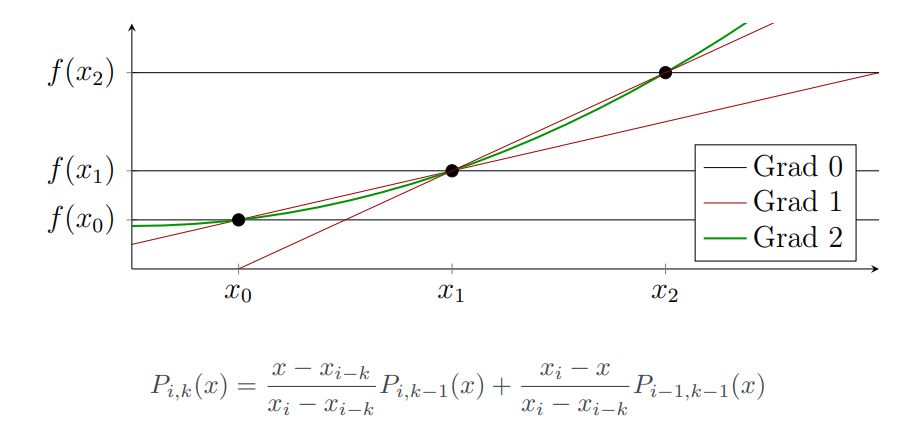
\includegraphics[scale=0.5]{assets/aikten_neville.png}
\end{center}
We want $T_{i,k} = P_{i,k}(0)$ so deriving that we get
\begin{itemize}
  \item $x = 0$
  \item $h_i = 2^{-i}h$
  \item $x_i = h_i^2 = 4^{-i}h^2$
\end{itemize} 
So if we substitute we achieve the Roberg Quadrature below
\subsubsection{Romberg Quadrature}
Aikten-Neville for the Romberg Quadrature: $T_{i,0} := T(2^{-i}h)$ for $i=0,1,2,..$ and
\[T_{i,k} := \frac{4^kT_{i,k-1} - T_{i-1,k-1}}{4^k -1}, \quad k=1,2,\dots, i=k,k+1,...\]
$T_{i,k}$ is a Quadrature Rule with Error order $h^{2k+2}$.

The costs are
\[\sum_{i=0}^k \left(2^{i} \frac{b-a}{h} + 1\right) \in O(2^k h^{-1})\]
The in-place algorithm
\begin{lstlisting}[language=Python]
  for i=0,...,p:
    T[i]= T(2^(-i) * h)
  for k=1,...,p:
    for i=p,p-1,...,k:
      T[i] = (4^k * T[i] - T[i-1])/(4^k - 1)
\end{lstlisting}
\subsection{High-Dimensional Quadrature}
Here $f:[0,1]\times[0,1] \to \mathbb{R}$, $(x,y) \to f(x,y)$

We want to compute an approximation for 
\[I(f) := \int_{y=0}^1 \left(\int_{x=0}^1 f(x,y) dx\right)dy\]
With quadrature rule $\tilde{I}$ for Function $[0,1] \to \mathbb{R}$

\[F(y) \approx \tilde{I}(x \to f(x,y)) = \sum_{j=0}^m c_j f(x_j,y)\]
That is on one dimension, we do something similar for the second one
\[I(f) \approx \tilde{I}(F) = \sum_{k=0}^m c_kF(y_k) \approx \sum_{k=0}^m\sum_{j=0}^m c_kc_j f(x_j,y_k)\]

The precision is $O(m^{-2})$, independent from $d$ (number of dimensions)

The time complexity is $O(m^{d})$
\subsection{Monte-Carlo Quadrature}
Having $\Omega \subseteq \mathbb{R}^d$ as the Ground space of a probability space $(\Omega, \mathcal{A}, \mathbb{P})$ with Uniform distribution $\mathbb{P}(A) = Vol(A) / Vol(\Omega)$ for all $A\in\mathcal{A}$

$f:\Omega \to \mathbb{R}$ Random variable with existing expected value
\[\mathbb{E}(f) = \int_\Omega f(x)dx\]
and Variance $\mathbb{V}(f)$

We pick $N$ independente random points $x_i$ and evaluate them
\[\overline{f} := \frac{1}{N} \sum_{i=1}^N f(x_i)\]
The expected value persists $\mathbb{E}(\overline{f}) = \mathbb{E}(f)$ and the variance is $\mathbb{V}(\overline{f}) = \frac{1}{N} \mathbb{V}(f)$

So we can think of $\overline{f}$ as an approximation to the integral with 'accuracy' $\sqrt{\mathbb{V}(\overline{f})} \in O(\sqrt{1/N})$
\section{Ordinary Differential Equation (ODE)}

Describe a function $\mathbb{R}\to \mathbb{R}$ through it's derivative.

Example: Position $s(t)\in\mathbb{R}$ of a biker at time point $t$.

If we know $s$, we can compute the velocity
\[v(t) = s'(t) = \frac{d}{dt}s(t)\]

But if we know $v(t)$ and the position at time point $s(0)$.

\[s(t) = s(0) + \int_{0}^t v(\tau)d\tau\]

And the differential equation is computing $s$ through relationship
\[s'(t) = v(t) = v(t,s)\]
Basically this translates to, the velocity depends not only on the time, but on the position.

\begin{center}
  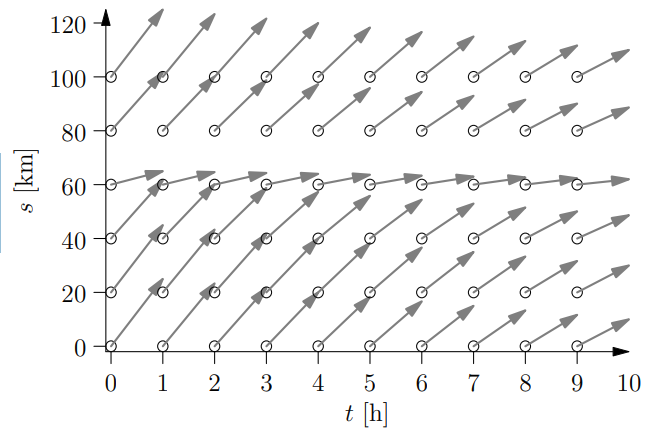
\includegraphics[scale=0.5]{assets/differential_equation.png}

  The velocity decreases through time if $s$ is constant. And velocity has a Gaussian form if $t$ stays constant. Like there is a steep hill at the middle point in the example of riding the bycicle.

  In the image, the length of the arrows is always picked so that $t = 1h$ always. This means the arrow at (0,0), in one hour we would travel around 25km 

  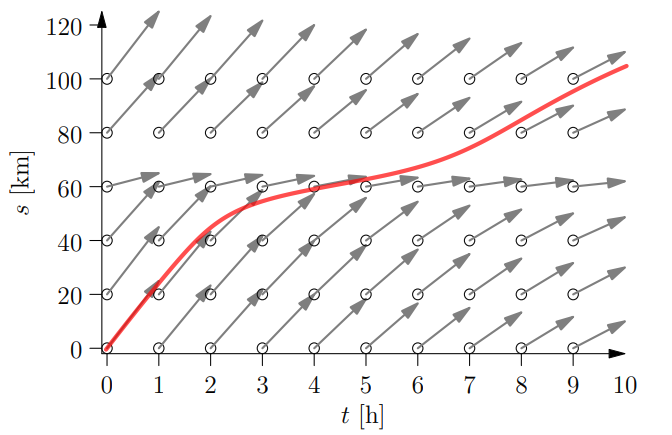
\includegraphics[scale=0.5]{assets/differential_equation_2.png}

  Result assuming $s(0) = 0$
\end{center}

\subsection{Formal Definition}
The ordinary differential equation (ODE) for a function $y:[t_0,T] \to \mathbb{R}$ ($t_0$ start time, $T$ end time) is an equation in the form
\[y'(t) = f(t,y(t))\]
with the RHS $f:[t_0,T]\times \mathbb{R}\to\mathbb{R}$

With an ODE and a start condition
\[y(t_0) = y^0\]
($y_0\in\mathbb{R}$) we get an \textbf{initial-value problem}

A differential equation is called \textbf{autonomous}, if $f(t,y)$ only depends on the second parameter $y$. So that the parameter $t$ does not have a direct impact, but only through $y(t)$

\subsection{Unordinary Differential Equations?}
The definition can easily be extended to use more equations $y:[t_0,T] \to \mathbb{R}^m$ or equations in higher derivatives of $y$. These are all still ODE.

Instead of start points $t=t_0$, we can distribute conditions on $t=t_0$ and $t=T$. These are called \textbf{boundary value problems}. These are however, still ODE's

However, if we use function with multiple variables $y:\Omega \subseteq \mathbb{R}^2 \to \mathbb{R}$. We build equations with partial derivatives, e.g

\[\frac{\partial^2}{\partial x_1^2}y(x_1,x_2) + \frac{\partial^2}{\partial x_2^2}y(x_1,x_2) = 0\]
These are called \textbf{partial differential equations}, 

\subsection{Example}
Let's have
\[y'(t) = -\lambda y(t)\]
It's homogenous, because $t$ doesn't appear directly.

For all $c\in\mathbb{R}$ the differential equation is solved by
\[y(t) = ce^{-\lambda t}\]


With the start condition $y(t_0) = y^0$ we get $c = y^0 /e^{-\lambda t_0}$

With that we have a full solution
\[y(t) = \frac{y^0e^{-\lambda t}}{e^{-\lambda t_0}} = y^0 e^{-\lambda \underbrace{(t-t_0)}_{\text{autonomous}}}\]
for the initial-value problem $y'(t) = -\lambda y(t)$, $y(t_0) = y^0$

We still don't know the uniqueness of the solution

NOTE: There is a cool example in the slides 'Populationsdynamik'

\subsection{Uniqueness of the solution}
The idea is that no two lines can 'cross', because if they crossed, they must have same position AND same time. Meaning it would have the same velocity, so they must be the same line.

This is proved in the Picard-Lindelöf Theorem. If $f(t,s)$ is continuous in $t$ and differentiable in $s$, then through each point $(t,s)$ there is only one solution curve $s(t)$.

\subsection{Simple One-Step Procedures}
From now on, the syntax will always be
\[y'(t) = f(t,y(t)) \quad y(t_0) = y^0\]

\subsubsection{Discretization and relation to quadrature}
We pick time points $t_0 < t_1 < ... < t_n = T$. Here equidistant with $n$ intervals $h = (T-t_0)/n$. We also know $f$.

We want to approximate the solution curve $y(t)$ with discrete points $y^k \approx y(t_k)$

The function
\[y(t) = y^0 + \int_{t_0}^t f(s,y(s))ds = y^0 + \sum_{j=0}^{n-1}\int_{t_j}^{t_{j+1}}f(s,y(s))ds\]
solves to initial-value problem (because if we derivate $f(s,y(s))$ and set $t=t_0$ we get $y_0$).

For each time step we use an appproximation $y^{j+1} := y^j + \Delta y^j$

With
\[\Delta y^j \approx \int_{t_j}^{t_{j+1}}f(s,y(s))ds\]

We approximate $y(s)$ by first solving the ODE with initial value  $y(t_j) = y^j$

Input values for a time step
\begin{itemize}
  \item Previous time step $t_j$ and time step width $t_{j+1} - t_j$
  \item $y^j \approx y(t_j)$
  \item RHS $f$ as a function 
\end{itemize}
The next approximation
\begin{itemize}
  \item Replace integral with Quadrature formula (weighted sum from evaluations of $f$ an certain points)
\end{itemize}

\subsubsection{Quadrature with rectangle rule (from left)}
We use the \textbf{Explicit Euler Process}: Quadrature rule with evaluation at $t = t_j$

\[y^j + \int_{t_j}^{t_{j+1}}f(s,y(s))ds \approx y^{j+1} := y^j + h\cdot f(t_j, y^j)\]

\paragraph{Example}:
If we remember the example $y'(t) = -\lambda y(t)$ 

\[y^{j+1} = y^j - h\lambda y^j = (1-h\lambda)^{j+1}y^0\]

And we know the true evaluation is
\[y(t_{j+1}) = y^0 e^{-\lambda (j+1)h}\]

\subsubsection{Quadrature with rectangle rule (from right)}
We use now the \textbf{implicit Euler Process} : Evaluation at $t = t_{j+1}$

\[y^j + \int_{t_j}^{t_{j+1}}f(s,y(s))ds \approx y^{j+1} := y^{j} + hf(t_{j+1}, y^{j+1})\]

Now instead of a formula, it is an equation to solve in $y^{j+1}$ it can be harder or easier, depending on $f$.

It does have some advantages though.

\paragraph{Example}: Same example, $y'(t) = -\lambda y(t)$

\[y^{j+1} = y^j - h \cdot \lambda \cdot y^{j+1} \Rightarrow y^{j+1} = \frac{1}{1+h\cdot \lambda}y^j = \left(\frac{1}{1+h\lambda}\right)^{j+1}y_0\]

If we apply the Taylor-Expansion in $\varepsilon = 0$
\[\frac{1}{1+\varepsilon} = 1-\varepsilon + O(\varepsilon^2)\]

And we know the true evaluation is
\[y(t_{j+1}) = y^0 e^{-\lambda (j+1)h}\]

\subsubsection{Error Rate}
Given we are comparing a collection of discrete points and a function, our error rate is 
\[\max_{0\leq j \leq n} |y(t_j) - y^j|\]
A process is called \textbf{convergent} of order $p$, if this error is in $O(h^p)$.

There can be two error sources for $y^{j+1}$
\begin{itemize}
  \item The summed up error of the previous steps $y(t_j) - y^j$
  \item The error in $y^{j+1} = y^j + \Delta y^j$
  \[\Delta y^j \approx \int_{t_j}^{t_{j+1}}f(s,y(s))ds\]
\end{itemize}
Luckily it is enough to just look at the second source.

\subsubsection{Consistency}
From the point $(t_j,y^j)$ we can go one time step forward. In the real function the value is $y(t_{j+1})$. Through our process we get $y^{j+1}$

So we call the \textbf{consistency error}:
\[\tau_{j,h} = \frac{y(t_{j+1}) - y^{j+1}}{h}\]
The process is consistent in order p, if $\tau_{j,h} \in O(h^p)$

We don't need too many restrictions of $f$ to say
\[\text{Consistency of order } p \Rightarrow \text{Convergence of order }p\]

\paragraph{Consistency of the explicit Euler Process}: Using the taylor expansion
\[y(t_{j+1}) = y(t_j) + hy'(t_j) + h^2\frac{y''(t_j)}{2} + O(h^3) \quad \text{ using n = 2}\] 
And with Euler
\[y^{j+1} = y(t_j) + hf(t_j,y(t_j)) = y(t_j) + hy'(t_j)\]
So
\[\tau_{j,h} = \frac{h}{2}y''(t_j) + O(h^2)\]

So the explicit (and also implicit) Euler Process is 
\begin{itemize}
  \item Consistent
  \item For flat enough $f$ ($f$ is w.r.t $y$ continously differentiable) convergent of Order $1$
\end{itemize}

\paragraph{Instability of the explicit Euler Process}: 
If we set $y'(t) = -\lambda y(t)$, with start value $y(0) = y^0$

The exact solution is
\[y(t)= y^0 e^{-\lambda t}\]

The explicit euler process gives us
\[y^{j} = y^{j+1} + h (-\lambda y^{j-1}) = y^0 (1-h\lambda)^j\]
So it is curious, our approximation varies wildly depending on the value of $h\lambda$

\begin{center}
  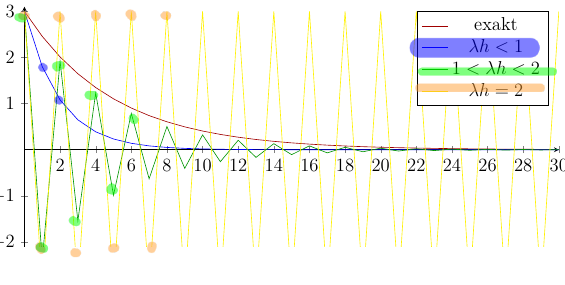
\includegraphics[scale=0.5]{assets/instability_euler_process.png}
  
  This behaviour is called the \textbf{instability}
\end{center}

\subsection{Higher Order ODE's}
The idea is somewhat nesting this processes, mixing with quadrature rules and such.

\subsubsection{Trapezoid method $m=2$}
If we integrate using the trapezoid rule
\[\int_{t_j}^{t_{j+1}}f(s,y(s))ds \approx \frac{h}{2}\left(f(t_j,y(t_j)) + f(t_{j+1},y(t_{j+1}))\right)\]
And we set $y(t_j) = y^j$ and $y(t_{j+1}) \approx y^{j+1}$
\[y^{j+1} = y^j + \frac{h}{2}\left(f(t_j,y^j) + f(t_{j+1},y^{j+1})\right)\]
This a second order process, but implicit. Can we make an explicit process?

\subsubsection{Process from Heun}
The idea is staying with the Trapezoid rule, but approximating $y(t_{j+1})$. We don't approximate it through $y^{j+1}$, but through the result of the explicit Euler Process
\[\tilde{y}^{j+1} = y^j + hf(t_j,y^j)\]
\[y^{j+1} = y^j + \frac{h}{2}\left(f(t_j,y_j) + f(t_{j+1}, \tilde{y}^{j+1})\right)\]
So we have an explicit second order process!

\subsubsection{Generalized Principle: Runge-Kutta Process}
It's an iterative method, where for a one-step method with $m$ evaluations of the right hand side $f$, we use 
\begin{itemize}
  \item Evaluation points $s_l = t_j + \alpha_l h$, with $0 \leq \alpha_l \leq 1$
  \item Approximations $u_l \approx y(s_l)$
  \item Auxiliary Directions $k_l = f(s_l,u_l)$
\end{itemize}

We use these to compute the quadrature weights $\gamma_l$ of the time step.
\[y^{j+1} = y^j + h \sum_{l=1}^m \gamma_lk_l\]

For the $u_i$ we construct analogous sums with quadrature weights $\beta_{i,l}$

\[u_i := y^j + h\sum_{l=1}^m\beta_{i,l}k_l \approx y^j + \int_{t_j}^{s_i} f(s,y(s))ds\]
\end{document}
